%//------ Section 03 -------------------------------------------------------------------------------------------------
\chapter{Mass measurements of multi-strange baryons in pp collisions at \sqrtS = 13 TeV}
\label{chap:CPTAnalysis}
%//-----------------------------------------------------------------------//

The first analysis conducted in this thesis aims at measuring the \rmXiM, \rmAxiP, \rmOmegaM, \rmAomegaP masses and mass differences between particle and anti-particle. This chapter provides a description of the different elements needed for its achievement. 


\section{Introduction}

%Symmetries certainly stand as one of the most fruitful concepts in Physics. They are of two kinds: continuous --- such as the global translations in both space and time, or the Lorentz transformations --- and discrete --- for example, the space- (P) and time- (T) inversions, the charge conjugation (C), and their combined transformation given by CPT. In particular, the Lorentz and CPT symmetries are connected by the so-called CPT theorem which states that any local Lorentz-invariant quantum field theory must also (under some extra requirements) be CPT invariant \cite{cptstatus}. Consequently, the CPT violation implies the breaking of the Lorentz symmetry, and vice versa\footnote{In fact, there is another option; to allow for CPT to be violated, either the Lorentz symmetry must be broken -- as in the string theory \cite{string} or the Standard-Model Extension \cite{sme} -- or some of the other extra assumptions of the CPT theorem must be dropped, namely the energy positivity, local interactions, finite spin, etc \cite{cptimplieslorentz}\cite{cptsymmetryantitsviolation}. } \cite{sozzi}. Another implication involves the relation between the properties of matter and antimatter: due to the charge conjugation linking particles to antiparticles, the CPT symmetry imposes that they share the same invariant mass, energy spectra, lifetime, coupling constants, etc \cite{cptsymmetryantitsviolation}. Most of the experimental checks of CPT invariance stem from these physical consequences.

As discussed in \Sec\ref{subsec:Theory}, the Standard Model is built upon a set of symmetries, each being either discrete -- such as the combination of the charge conjugation (C), parity (P) and time reversal (T), known as the CPT transformation -- or continuous -- for example, the Lorentz transformations that includes rotations and boosts. In particular, the Lorentz and CPT symmetries are connected by the so-called CPT theorem which establishes that any unitary, local Lorentz-invariant quantum field theory must be CPT invariant \cite{kosteleckyStatusCPT1998}. Consequently, the CPT violation implies the breaking of the Lorentz symmetry, and vice versa\footnote{In fact, another option exists; to allow for the CPT violation, either the Lorentz symmetry must be broken -- as in the case of string theory \cite{kosteleckySpontaneousBreakingLorentz1989} or the Standard-Model Extension \cite{colladayLorentzviolatingExtensionStandard1998} -- or some of the other additionnal assumptions of the CPT theorem must be dropped, namely the energy positivity \cite{abersDiseasesInfiniteComponentField1967}, local interactions \cite{carruthersIsospinSymmetryTCP1968}, finite spin \cite{oksakInvalidityTCPtheoremInfinitecomponent1968}, etc \cite{greenbergCPTViolationImplies2002}\cite{lehnertCPTSymmetryIts2016}. } \cite{sozziTestsDiscreteSymmetries2019}. Another implication involves the relation between the properties of matter and antimatter: due to the charge conjugation linking particles to antiparticles, the CPT symmetry imposes that they share the same invariant mass, energy spectra, lifetime, coupling constants, etc \cite{cptsymmetryantitsviolation}. Most of the experimental checks of CPT invariance stem from this last point, which imposes several constraints on the anti-particle properties. \\

The Particle Data Group (PDG) \cite{particledatagroupReviewParticlePhysics2022} compiles a large variety of CPT tests from many experiments and with different degrees of precision; so far, no CPT violation have been observed. The most stringent test involves the \rmKzero-\rmAKzero mixing process, which depends on the mass and lifetime differences of these two states. In this way, assuming no other source of CPT violation in the decay of neutral kaons, these two quantities have been bounded \cite{particledatagroupReviewParticlePhysics2022}\cite{angelopoulosK0K0Mass1999} to 

\begin{equation}
2 \frac{\mid m_{\rmKzero} - m_{\rmAKzero} \mid}{m_{\rmKzero} + m_{\rmAKzero}} < 6 \times 10^{-19} \quad , \quad 2 \frac{\mid \Gamma_{\rmKzero} - \Gamma_{\rmAKzero} \mid}{\Gamma_{\rmKzero} + \Gamma_{\rmAKzero}} = (8 \pm 8) \times 10^{-18}.
\end{equation}

These indirect limits are much stronger than the ones extracted from direct tests. For example, in the hyperon sector, the precision on relative mass difference is typically of a few $10^{-5}$. In the latter case, it should be mentioned that there is still some room for improvements, and most particularly concerning the mass difference measurements between particle and anti-particle in the multi-strange baryon sector. The only test of this nature dates back to 2006 \cite{abdallahMassesLifetimesProduction2006} for the \rmXiM and \rmAxiP, and from 1998 \cite{chanMeasurementPropertiesOverline1998} for the \rmOmegaM and \rmAomegaP. The former was achieved by exploiting 3.25 million hadronic decays of the \rmZzero recorded by the DELPHI detector at LEP-1; the latter was obtained on the E756 spectrometer at Fermilab, using an 800 \gmom proton beam on a beryllium target. However, both studies suffer from low statistics: approximately 2500(2300) reconstructed \rmXiM (\rmAxiP) and about 6323(2607) reconstructed \rmOmegaM (\rmAomegaP) were used.\\

\begin{table}[t]
    \centering
    \begin{tabular}{>{\centering\arraybackslash}b{1.5cm}@{\hspace{0.3cm}} >{\centering\arraybackslash}b{1.75cm}@{\hspace{0.3cm}} >{\centering\arraybackslash}b{2.85cm}@{\hspace{0.3cm}} >{\centering\arraybackslash}b{3.6cm}@{\hspace{0.3cm}} >{\centering\arraybackslash}b{2.5cm}@{\hspace{0.3cm}} >{\centering\arraybackslash}b{1cm}@{\hspace{0.3cm}}}
    \noalign{\smallskip}\hline\noalign{\smallskip}
	Particle & Quark content & Mass (\mmass) & Relative mass difference & Dominant decay channel & B.R.\\	
    \noalign{\smallskip}\hline \noalign{\smallskip}
    	
	\rmKzeroS (\rmAKzeroS) & $d \bar{s}$ ($\bar{d} s$)& $497.611 \pm 0.013$ & $< 6 \times 10^{-19}$ & \piPlus \piMinus & 69.20\%\\
	
    \noalign{\smallskip}\hline \noalign{\smallskip}
    
    \rmLambda (\rmAlambda) & $u d s$ ($\bar{u}\bar{d}\bar{s}$) & $1115.683 \pm 0.006$ & $\left(-0.1 \pm 1.1\right) \times 10^{-5}$ & \proton \piMinus (\pbar \piPlus) & 63.9\% \\
    
    \noalign{\smallskip}\hline \noalign{\smallskip}    
    
    \rmXiM (\rmAxiP) & $dss$ ($\bar{d}\bar{s}\bar{s}$) & $1321.71 \pm 0.07$ & $\left(-2.5 \pm 8.7\right) \times 10^{-5}$ & \rmLambda \piMinus (\rmAlambda \piPlus) & 99.9\% \\	
    \noalign{\smallskip}\hline \noalign{\smallskip}
    
	\rmOmegaM (\rmAomegaP) & $sss$ ($\bar{s}\bar{s}\bar{s}$) & $1672.45 \pm 0.23$ & $\left(-1.44 \pm 7.98\right) \times 10^{-5}$ & \rmLambda \rmKminus (\rmAlambda \rmKplus) & 67.8\%\\    
    \noalign{\smallskip}\hline\noalign{\smallskip}
    \end{tabular}
    \caption{A few characteristics, as of 2023, of the \rmLambda, \rmXi, \rmOmega hyperons and the \rmKzeroS meson: quark content, mass, relative mass difference values with their associated uncertainties and their dominant decay channel as well as the corresponding branching ratio \cite{particledatagroupReviewParticlePhysics2022}.}\label{tab:V0CascPDGMass}
\end{table}

In comparison, all the pp collisions at a centre-of-mass energy of 13 \tev collected by ALICE throughout the LHC Run-2 contains about 2 400 000 \rmXi and 129 000 \rmOmega, with little background. Therefore, in this thesis, the measurement of the mass difference of \rmXiM and \rmAxiP, and \rmOmegaM and \rmAomegaP hyperons is performed. It relies on data samples much larger than those exploited previously. These direct measurements of the mass difference offer a test of the CPT invariance to an unprecedented level of precision in the multi-strange baryon sector. The absolute masses are updated as well, with a precision substantially better than the current values listed in the PDG and presented in the \tab\ref{tab:V0CascDecay}.

Furthermore, concerning the \rmLambda hyperon and \rmKzeroS meson, the PDG quotes a precision of a few \kmass on the mass value, and about $1 \times 10^{-5}$ on the relative mass difference value\footnote{This only concerns the relative mass difference between \rmLambda and \rmAlambda. As mentioned above, such quantity is much smaller by fourteen orders of magnitude in the case of \rmKzero.}. Abundantly produced, these two hadrons also exhibit an irresistible feature in the context of this thesis: both decay into a V0 in their dominant decay channel, and so can be identified in a similar manner as cascades using topological reconstruction. For those two reasons -- high precision on the PDG mass values, and similar decay topology as cascade --, the analysis is reproduced on \rmLambda and \rmKzeroS, both being used as a benchmark for the measurement.\\

In the following, the term \textit{mass difference} always refers to the relative one, namely $(\mMassApart{part.} - \mMassPart{part.})/\mMassPart{part.}$, unless indicated otherwise.

\section{Data samples and event selection}

\subsection{The data samples}

All the data samples employed for this measurement originates from the second campaign of data taking, the LHC Run-2. The latter comprises different collision systems at various energies, mainly pp collisions at \sqrtS = 13 \tev and Pb-Pb collisions at \sqrtSnn = 5.02 \tev. Based on the elements in \Sec\ref{subsec:HyperonAndALICE}, the analysis exploits the former ones as they provide a less dense collision environment, expectedly easier to reconstruct and thus more controllable. All these pp events have been collected during three data taking periods: between April and October 2016, May and November 2017, April and October 2018 (\Sec\ref{subsec:acceleratorprogramme}, \tab\ref{tab:LHCRunProgramm}).

Considering the target precision on the mass and mass difference values, it is crucial to have a fine comprehension of the data reconstruction to keep it well under control. For that reason, the analysis uses data in ESD format as they contain all the informations related to event building, thus offering the possibility to replay \textit{offline} the V0 and cascade vertexings/formations. As mentioned in \Sec\ref{subsubsec:DataFormats}, the first full reconstruction cycle (\Sec\ref{subsubsec:computingmodel}), performed right after their recording of the data, produces ESD files labelled as \textit{pass-1}. Since then, other reconstruction cycles have been carried out, each iteration bringing its share of improvements or fixes. The events analysed for this measurement originates from the second reconstruction cycle, the pass-2, which offers better tracking performances: same version of analysis software over all the data taking periods leading to more uniform performances, better SPD and TPC alignments, improved TPC reconstruction and finer description of the distortions within the TPC gas.

Each period consists in fact of dozens or hundreds of \textit{runs}, corresponding to sequences of events recorded in an uninterrupted manner\footnote{Throughout the data taking, it is more or less frequent to interrupt the data collection, \ie stop the run. This usually occurs when a detector encounters an error, unfixable while collecting data. Broadly speaking, a period regroups a set of runs that have been recorded within the same data taking conditions.}. The lists of approriated runs for physics analysis are defined by the ALICE Data Preparation Group (DPG). As its name suggests, the latter oversees the preparation, reconstruction, quality assurance of both collected and simulated data, as well as the upkeep of the analysis tools including the event and track selections \cite{alicecollaborationALICEDataPreparation2023}. The list of runs employed in this study follows the DPG's one for an analysis using central barrel detectors and requiring hadron PID. For a run to be in that list, all the detectors related to the tracking and PID must be operational -- \ie SPD, SDD, SSD (ITS), TPC, TOF --, as well as those in charge of triggering, that are the V0 and T0. Note that it does not mean that the PID performances are optimal, nor that the full acceptance of each detector is covered.\\

Besides the real data sample, the measurement also relies on simulated data in order to estimate and optimize the performances of the analysis. To each run corresponds its simulated counterpart, anchored on pass-2 data, as described in \Sec\ref{subsubsec:MCData}. All the exploited MC productions employ \Pythiaeight (version 8.2, tune: Monash 2013) as event generator. For the transport and interaction with the material of the ALICE detector, most of them use \GeantThree; although \GeantFour runs faster, describes more accurately hadronic interactions at very low momentum and is better maintained, only a few of the exploited simulations rely on it \cite{barendsGeant4ValidationStudy2017}.

Since both abundant (\rmKzeroS, \rmLambda and to a certain extent, \rmXi) and rare species (\rmXi and \rmOmega) are being studied, one may resort to two kinds of simulations: general-purpose MC productions for the first ones, and enriched MC productions for the others. Here, the enriched simulations have been obtained by selecting the events that includes, at least, a \rmKzeroS, \rmLambdaPM, \rmXiPM or \rmOmegaPM in $\abspseudorap < 1.2$.

Furthermore, this analysis also makes use of the track references in the simulation. As mentioned in \Sec\ref{subsubsec:MCData}, these correspond to the MC informations of the considered track at the location where it crosses a given detection plane. Thereby, they allow to compare the reconstructed track informations with the actual/generated ones at any point along the particle trajectory\footnote{Strictly speaking, this comparison cannot be done at any point since the track reference is only available where the particle traverses a sensitive volume.}. Although the track references are effectively stored for only 10\% of the production\footnote{This is done in order to spare some disk space.}, this comparison is proving invaluable to control the tracking in ALICE.\\


In total, the exploited data sample counts about 2.6 billions minimum bias events at \sqrtS = 13 \tev, and approximately 600 millions events in the associated MC productions.

\subsection{The event selection}

As mentioned in \Sec\ref{subsec:TriggerSystem}, the analysis focuses on minimum-bias and/or high-multiplicity events. More precisely, the respective trigger configurations correspond to the MB$_{\rm AND}$ and/or HM$_{\rm VZERO}$. Not all the events passing these trigger selections are considered; additional cuts are applied in order to filter out only those of \say{good} quality for a physics analysis. \\

During the data acquisition (DAQ), the event-builder proceeds to the event reconstruction based on the sub-events from all contributing detectors. It may happen, however, that the detector's output can not be transmitted due to the associated data channel being closed\footnote{There are different reasons for the data channel to be closed. At the beginning or the end of each run, a specific procedure is performed on all detectors in order to effectively initiate the start or stop of the run. In particular, the \say{End Of Run} procedure has to close all the data channel connecting the event-builder and the sub-detectors -- \ie the GDCs and LDCs respectively (\Sec\ref{subsec:TriggerSystem}) --, but this termination can occur sooner in the case of a connection time-out for example.} \cite{alicecollaborationTriggerDataAcquisition}. The event-builder still reconstructs the event, although it is tagged as \say{incomplete DAQ} due to the missing informations. Such events are rejected in the present work.\\

There exists three types of reconstructed primary vertex in ALICE, from the highest to the poorest quality: one estimated using the global ITS-TPC tracks (\Sec\ref{subsubsec:FinalVertexDet}), another based on the SPD tracklets (\Sec\ref{subsubsec:PreliminaryVertex}), and the last built from the TPC standalone tracks in a similar way as the former. By default, only the \say{best} available reconstructed primary vertex is considered. 

Nevertheless, to ensure that the event has a vertex of a sufficiently good quality, the analysis relies exclusively on the first two aforementioned primary vertices. This boils down to requiring the presence of, at least, the one reconstructed using tracklets\footnote{As mentioned in \Sec\ref{subsubsec:PreliminaryVertex}, the event cannot be built without the primary vertex based on SPD tracklets. Hence, by construction, the presence of such vertex is guaranteed in the event.}. Moreover, the resolution of the latter in the longitudinal direction should not exceed 0.25 \cm. In cases when both SPD tracklets and global ITS-TPC track vertices are available, their positions along the beam axis must coincide within a 0.5 \cm window.

As a prerequisite for guaranteeing an uniform reconstruction efficiency, particles must remain within the acceptance of all the central detectors involved in their reconstruction, that is $\abspseudorap < 0.9$. For particles originating from the interaction point, this condition implies a constraint on the longitudinal position of the primary vertex: the distance between the interaction point and the centre of ALICE should be below 10 \cm along the beam axis\footnote{Note that there is no selection of such nature concerning the transverse position of the primary vertex, except that it must be located below the beam pipe.}. \\

A key element of the event quality concerns the pile-up level. The latter occurs when there are two or more collisions coming from the same bunch crossing -- this is the \textit{in-bunch} pile-up -- and/or from different bunch crossings occuring within the readout time of the detectors -- also called \textit{out-of-bunch} pile-up. One approach to remove both types of pile-up consists in rejecting events with multiple reconstructed primary vertices. This selection depends on the nature of the best primary vertex available.
\begin{itemize}
\item[$\bullet$] If it is the one reconstructed using ITS-TPC tracks, the event selection algorithm checks the presence of another vertex of reasonably good quality ($\rmChiSquareNDF < 5$, with $NDF$ the number of degree of freedom), formed out of at least five tracks, and separated from the first one by more than $15 \sigma$\footnote{Here, $\sigma$ denotes the uncertainty on the distance between the two vertices.}. If such vertex exists, the event is discarded. 
\item[$\bullet$] Otherwise, it corresponds to the one built from SPD tracklets. To maximise the selection efficiency, the cuts adapt to the tracklet multiplicity. Hence, if a second vertex is found to be away from the first one by more than 0.8 \cm along the beam axis, with at least three, four or five associated tracklets for a total number of reconstructed tracklets (\rmNTracklet) inferior to 20, $20 < \rmNTracklet \leq 50 $ and \rmNTracklet > 50 respectively, then the event is rejected.
\end{itemize}


Along the same line, the two innermost layers of the ITS can help to identify the remaining beam-induced background -- that have not been removed by the MB$_{\rm AND}$ trigger selection -- and pile-up events. As mentioned in \ref{subsubsec:PreliminaryVertex}, a tracklet is formed out of pair of clusters found in the two SPD layers, separated by an angle of 0.01 rad at most. Therefore, the number of clusters increases, so does the amount of reconstructed tracklet. However, in the case of beam-gas event, there should be many clusters but only a small number of tracklets could be formed using the previous definition. In pile-up events, only the tracklets associated with the primary vertex are considered; for that reason, the number of clusters should be relatively larger than expected at such tracklet multiplicity \cite{alicecollaborationALICEPhysicsForum2016}. In this way, based on this correlation between the number of SPD clusters and tracklets, the remaining events flagged as background or pile-up are rejected. \\

\begin{figure}[t]
	\centering
	\includegraphics[width=1\textwidth]{Figs/Chapter5/EventSelection.eps}
	\caption{Fraction of rejected events in the present data sample for each event selection: trigger selections (MB$_{\rm AND}$ and/or HM$_{\rm VZERO}$), incomplete DAQ, consistency between the global track and SPD tracklet vertices, longitudinal position of the primary vertex ($\mid \Delta z \mid < 10 $ \cm), pile-up removal for ITS-TPC track and SPD tracklet vertices, correlation between SPD tracklets and clusters.}
	\label{fig:EvtSelection}
\end{figure}


The \fig\ref{fig:EvtSelection} provides the fraction of rejected events as a function of the above selections in pp collisions at \sqrtS = 13 \tev.

\section{Analysis of the hyperon masses}

\subsection{Track selections}
\label{subsec:TrackSelections}

The identification of V0s and cascades strongly depends on the quality of the daughter tracks, and more precisely on their momentum resolution and trajectory. For that reason, the strange particle reconstruction relies exclusively on ITS-TPC combined tracks, since they offer the best momentum resolution as discussed in \Sec\ref{subsubsec:TrackReco} and shown in \fig\ref{fig:MomResolution}. In order to ensure an excellent momentum resolution as well as a fine estimation of the particle trajectory, various selection criteria are applied on the daughter tracks.\\

The analysis concentrates exclusively on tracks comprised within the pseudo-rapidity region $\abspseudorap < 0.8$. The latter corresponds to the acceptance volume of all the central detectors, which provides a flat reconstruction efficiency. Moreover, any track containing ITS and/or TPC shared clusters is rejected, as they potentially correspond to wrongly assigned clusters that could bias the tracking quality. 

Tracks belonging to a \textit{kink} vertex are discarded from the analysis, as they most certainly do not originate from a cascade decay and thus represent an additional source of combinatorial background. A kink usually happens when a charged particle decays into a neutral and a charged particle, such as $\Kplusmin \rightarrow \piZero \rmPiPM$. The former being undetected, they are identified by forming pairs of tracks, that intersect in space with a large angle and share the same electric charge.

Each track should have passed the final refit in the TPC. This means that its parameters have been estimated successfully in the TPC during the third stage of the tracking, when the track is propagated inwards to their distance of closest approach to the primary vertex (\Sec\ref{subsubsec:TrackReco}). To guarantee a good momentum resolution and a stable particle identification (PID) based on the energy deposit (\dEdx) in the TPC, the tracks need to be associated to at least 70 readout pad rows in the TPC out of 159 in total. These selections eliminate the contribution of short tracks and, incidentally, pairs of tracks formed out of the clusters from a single actual particle.\\

The reconstruction of V0s and cascades presented in \chap\ref{chap:V0CascReconstruction} does not resort to any kind of selections on the nature of the daughter particles, apart from their electric charge. This yields \textit{de facto} to an outstanding amount of background candidates. One way of suppressing the latter with a minimal cost in terms of signal candidates consists in using the PID informations provided by the TPC. In practice, the idea is to reject every association that involves tracks inconsistent with the expected identities for either a \rmKzeroS, \rmLambdaPM, \rmXiPM or \rmOmegaPM decay.

As explained in \Sec\ref{subsubsec:TPC}, a track can be labeled as a pion, proton or kaon by making use the PID estimator in \eq\ref{eq:PIDEstimator}, \Nsigma, which evaluates the difference between the measured \dEdx and the expected one under a given particle mass hypothesis in units of relative resolution. The separation power of such estimator evolves with the particle momentum which, in turn, influences the selection threshold and has some implications in terms of purity and efficiency: the tighter the selection on \Nsigma, the higher the purity but at the price of a small efficiency; conversely, a looser cut on \Nsigma deteriorates the purity in favour of a higher efficiency.

The identification strategy adopted here consists in selecting only the tracks compatible with their expected mass hypothesis within \Nsigma = $\pm 3$ at most. This selection is applied on each decay daughters, irrespective of their momentum or the one of the mother particle. This therefore imposes that:
\begin{itemize}
\item[$\bullet$] the bachelor track must consistent with the \rmPiPM or \rmKPM mass hypothesis, in the case of \rmXiPM or \rmOmegaPM respectively,
\item[$\bullet$] the positive track needs to be compatible with a proton hypothesis,
\item[$\bullet$] and the negative track has to agree with energy loss band of the pion.
\end{itemize}
Note that the last two constraints only allow to identify a \rmLambda and, associated with the bachelor track, a \rmXiM or \rmOmegaM. In order to select their anti-particle, one needs to swap the mass hypothesis of these two items, namely the positive track corresponds to a pion and the negative track, an anti-proton. For the \rmKzeroS, the particle is indistinguishable from the anti-particle in exploited V0 decay channel; both positive and negative tracks should be compatible with the pion hypthesis.


\subsection{V0s and cascades selections}
\label{subsec:V0CascSelections}

\subsubsection{Topological and kinematic selections}

Once the events and tracks have been selected, the topological reconstruction of V0s and cascades comes into play, as explained in \chap\ref{chap:V0CascReconstruction}. However, not all the candidates are considered in the analysis. As suggested in \Sec\ref{subsec:HyperonAndALICE}, ALICE is well suited for studying hyperons but only at mid-rapidity. This means that the V0s and cascades are reconstructed in the rapidity window $\absrap < 0.5$.

\begin{table}[t]
    \centering
    \begin{tabular}{c|c|c}
    \noalign{\smallskip}\hline \noalign{\smallskip}
    \bf Candidate variable & Selections \rmLambdaPM & Selections \rmKzeroS \\
    \noalign{\smallskip}\hline \noalign{\smallskip}    
    V0 \pT interval (\gmom) & \multicolumn{2}{c}{1 < \pT < 5} \\
    V0 rapidity interval & \multicolumn{2}{c}{\absrap < 0.5} \\
    Competing mass rejection (\gmass) & > 0.010 & > 0.005 \\
    MC association (MC only) & \multicolumn{2}{c}{Correct identity assumption} \\ 

    \noalign{\smallskip} \hline \noalign{\smallskip}
    \bf Track variable & Selections \rmLambdaPM & Selections \rmKzeroS \\
    \noalign{\smallskip} \hline \noalign{\smallskip}
    Pseudo-rapidity interval & \multicolumn{2}{c}{\abspseudorap < 0.8} \\
    TPC refit & \multicolumn{2}{c}{\CheckGr} \\
    Nbr of crossed TPC readout rows & \multicolumn{2}{c}{ > 70} \\
    $\Nsigma^{\rm TPC}$ & \multicolumn{2}{c}{< 3} \\
    \multirow{ 2}{*}{Out-of-bunch pile-up rejection} & \multicolumn{2}{c}{at least one track with} \\
     & \multicolumn{2}{c}{ITS-TOF matching} \\
    
    \noalign{\smallskip}\hline \noalign{\smallskip}
    \bf Topological variable & Selections \rmLambdaPM & Selections \rmKzeroS \\
    \noalign{\smallskip}\hline \noalign{\smallskip}
    
    V0 decay radius (\cm) & \multicolumn{2}{c}{> 0.5}\\
    V0 Lifetime (\cm) & \multicolumn{2}{c}{< 3 $\times$ \cTau}\\
    V0 cosine of pointing angle & \multicolumn{2}{c}{> 0.998}\\
    DCA proton to prim. vtx (\cm) & > 0.06 & \NoWay \\
    DCA pion to prim. vtx (\cm) & \multicolumn{2}{c}{> 0.06} \\
%    DCA V0 to prim. vtx (\cm) & < 1 & < 0.06 \\
    DCA between V0 daughters (std dev) & \multicolumn{2}{c}{< 1} \\
    
    \noalign{\smallskip}\hline \noalign{\smallskip}
    \end{tabular}
    \caption{Summary of the topological and track selections, as well as the associated cut values, used in the reconstruction of \rmLambdaPM and \rmKzeroS in pp events at \sqrtS = 13 \tev. The \textit{competing mass rejection} refers to the removal of the background contamination from other mass hypotheses (\Sec\ref{subsubsec:InvariantMassSelection}). In the \rmLambdaPM case, this consists in comparing the invariant mass under the assumption of a \rmPiPlus\rmPiMinus and PDG mass of \rmKzeroS, that is the quantity $\mid\mInv{\rm hyp.\ \rmKzeroS} - \mPDG\rmKzeroS|$. When reconstructing \rmKzeroS candidates, the selection variable becomes $\mid\mInv{\rm hyp.\ \rmLambda} - \mPDG\rmLambda|$.}\label{tab:V0Selections}
\end{table}

The above selections on the track quality in TPC exclude the possibility of studying the particles of interest at low momentum ($\pT \leq 0.6$ \gmom). At such values, the V0s and cascades decay into very low momentum tracks, that can only be reconstructed via the ITS standalone tracking. Even when these tracks reach the TPC, they form short tracks and are thus rejected (\Sec\ref{subsec:TrackSelections}). As a matter of fact, in order to secure a reasonably good momentum resolution on the decay daughters, this analysis only considers candidates from 1 to 5 \gmom. On one hand, the \eq\ref{eq:Gluckstern} indicates that the momentum resolution deteriorates at low momentum ($\pT \leq 1$ \gmom) due to their relatively \say{short} track length, \say{small} number of clusters and the dominant contribution of multiple scattering. On the other hand, at high \pT ($\pT \geq 5$ \gmom), the resolution also decreases as a consequence of less pronunced track curvature.\\

To further remove the contribution from out-of-bunch pile-up events, it is required for at least one of the daughter tracks to either have a cluster in the innermost ITS layers\footnote{Technically, it is requested to have passed the final refit in the ITS and to have a hit in one of the two SPD layers.} or match with a hit in the TOF. The former uses the fast readout time of the SPD to limit the pile-up to tracks produced in collisions within $\pm$ 300 \nsec, that is twelve bunch crossings; the latter exploits the highly precise timing information of the TOF to identify the bunch crossing from which the particle originates, with an efficiency of approximately 70 to 80\% for intermediate or high \pT particles and drops rapidly for lower momentum due to mismatches \cite{alicecollaborationALICEDPGPileup}. This selection has been thoroughly studied in the context of a strange particle production analysis \cite{alicecollaborationMultiplicityDependenceMulti2020}; it was shown that applying this ITS-TOF matching condition on at least one of the decay daughters is sufficient to eliminate most of the remaining pile-up contamination.\\

\begin{table}[t]
    \centering
    \begin{tabular}{c|c|c}
    \noalign{\smallskip}\hline \noalign{\smallskip}
    \bf Candidate variable & Selections \rmXiPM & Selections \rmOmegaPM \\
    \noalign{\smallskip}\hline \noalign{\smallskip}    
    Cascade \pT interval (\gmom) & \multicolumn{2}{c}{1 < \pT < 5} \\
    Cascade rapidity interval & \multicolumn{2}{c}{\absrap < 0.5} \\
    Competing mass rejection (\gmass) & \NoWay & > 0.008 \\
    MC association (MC only) & \multicolumn{2}{c}{Correct identity assumption} \\ 

    \noalign{\smallskip}\hline \noalign{\smallskip}
    \bf Track variable & Selections \rmXiPM & Selections \rmOmegaPM \\
    \noalign{\smallskip}\hline \noalign{\smallskip}
    Pseudo-rapidity interval & \multicolumn{2}{c}{\abspseudorap < 0.8} \\
    TPC refit & \multicolumn{2}{c}{\CheckGr} \\
    Nbr of crossed TPC readout rows & \multicolumn{2}{c}{ > 70} \\
    $\Nsigma^{\rm TPC}$ & \multicolumn{2}{c}{< 3} \\
    \multirow{ 2}{*}{Out-of-bunch pile-up rejection} & \multicolumn{2}{c}{at least one track with} \\
     & \multicolumn{2}{c}{ITS-TOF matching} \\
    
    \noalign{\smallskip}\hline \noalign{\smallskip}
    \bf Topological variable & Selections \rmXiPM & Selections \rmOmegaPM \\
    \noalign{\smallskip}\hline \noalign{\smallskip}
    
    \multicolumn{3}{l}{\textbf{V0}} \\
    V0 decay radius (\cm) & > 1.2 & > 1.1\\
    V0 cosine of pointing angle & \multicolumn{2}{c}{> 0.97}\\
    |$m$($V0$) - \mPDG\rmLambda| (\gmass) & \multicolumn{2}{c}{< 0.008} \\
    DCA proton to prim. vtx (\cm) & \multicolumn{2}{c}{> 0.03} \\
    DCA pion to prim. vtx (\cm) & \multicolumn{2}{c}{> 0.04} \\
    DCA V0 to prim. vtx (\cm) & \multicolumn{2}{c}{> 0.06} \\
    DCA between V0 daughters (std dev) & \multicolumn{2}{c}{< 1.5} \\
    \noalign{\smallskip}\hline \noalign{\smallskip}
    
    \multicolumn{3}{l}{\textbf{Cascade}} \\
    Cascade decay radius (\cm) & > 0.6 & > 0.5 \\
    Cascade Lifetime (\cm) & \multicolumn{2}{c}{< 3 $\times$ \cTau}\\
    DCA bachelor to prim. vtx (\cm) & \multicolumn{2}{c}{> 0.04} \\
    DCA between cascade daughters (std dev) & \multicolumn{2}{c}{< 1.3} \\
    Cascade cosine of pointing angle & \multicolumn{2}{c}{> 0.998} \\
    Bachelor-proton pointing angle (rad) & \multicolumn{2}{c}{> 0.04} \\
    
    \noalign{\smallskip}\hline \noalign{\smallskip}
    \end{tabular}
    \caption{Summary of the topological and track selections, as well as the associated cut values, used in the reconstruction of \rmXiPM and \rmOmegaPM in pp events at \sqrtS = 13 \tev. The \textit{competing mass rejection} refers to the removal of the background contamination from other mass hypotheses (\Sec\ref{subsubsec:InvariantMassSelection})}\label{tab:CascadeSelections}
\end{table}

In summary, the \tabs\ref{tab:V0Selections} and \ref{tab:CascadeSelections} provide a list of the track and topological selections employed in the reconstruction of V0s and cascades respectively, as well as the numerical cut values. Note the tight cut on the cosine of pointing angle of the cascade candidate; this is discussed later in \Sec\ref{subsec:MassExtraction}.

\subsubsection{Structure in the invariant mass spectrum of cascades}
\label{subsubsec:InvMassStructure}

Among the topological selections listed in \tab\ref{tab:CascadeSelections}, one of them has not been introduced and discussed in \chap\ref{chap:V0CascReconstruction}, namely the cut on the pointing angle formed by the bachelor and the positive particles. Contrarily to the other selections, this one is not standard in ALICE; it has been introduced in 2020 by \cite{silvadealbuquerqueMultistrangeHadronsPb2019}. At that time, a structure in the invariant mass distribution of \rmXi and \rmOmega, similar to the one in \figs\ref{fig:WrongPA}, was observed in Pb-Pb collisions. It turned out that the bump background, between 1.28 and 1.31 \gmass on \figs\ref{fig:XiMinusWrongPA} and \ref{fig:XiPlusWrongPA}, originates from an erroneous track association in the cascade reconstruction. 

A V0 decays into a baryon \proton/\pbar and a \rmPiMinus/\rmPiPlus, depending on whether this is a \rmLambda or \rmAlambda. In the situation where another negative/positive track in the event passes close by the proton/anti-proton, the reconstruction algorithm may interpret that as a V0 decay; this track plays the role of the negative/positive daughter particle of a \rmLambdaPM, and the proton/anti-proton corresponds to its positive/negative daughter particle. On the other hand, the \rmPiMinus/\rmPiPlus daughter of the actual \rmLambdaPM is combined to other particles, and most likely to the previously ill-formed V0. In such case, it acts like the bachelor particle of a cascade decay. In other words, while the actual topology is depicted in \fig\ref{fig:WrongV0}, it is reconstructed as a cascade, as illustrated in \fig\ref{fig:TrueV0}.

The analysis \cite{silvadealbuquerqueMultistrangeHadronsPb2019} investigated different strategies in order to remove this background contamination. In the end, the best option consists in rejecting candidates with a small pointing angle for the actual V0, \ie the pointing angle between the bachelor and the proton, as shown in \fig\ref{fig:WrongPACut}.


\begin{figure}[t]
\hspace*{-1.5cm}
\subfigure[]
{
	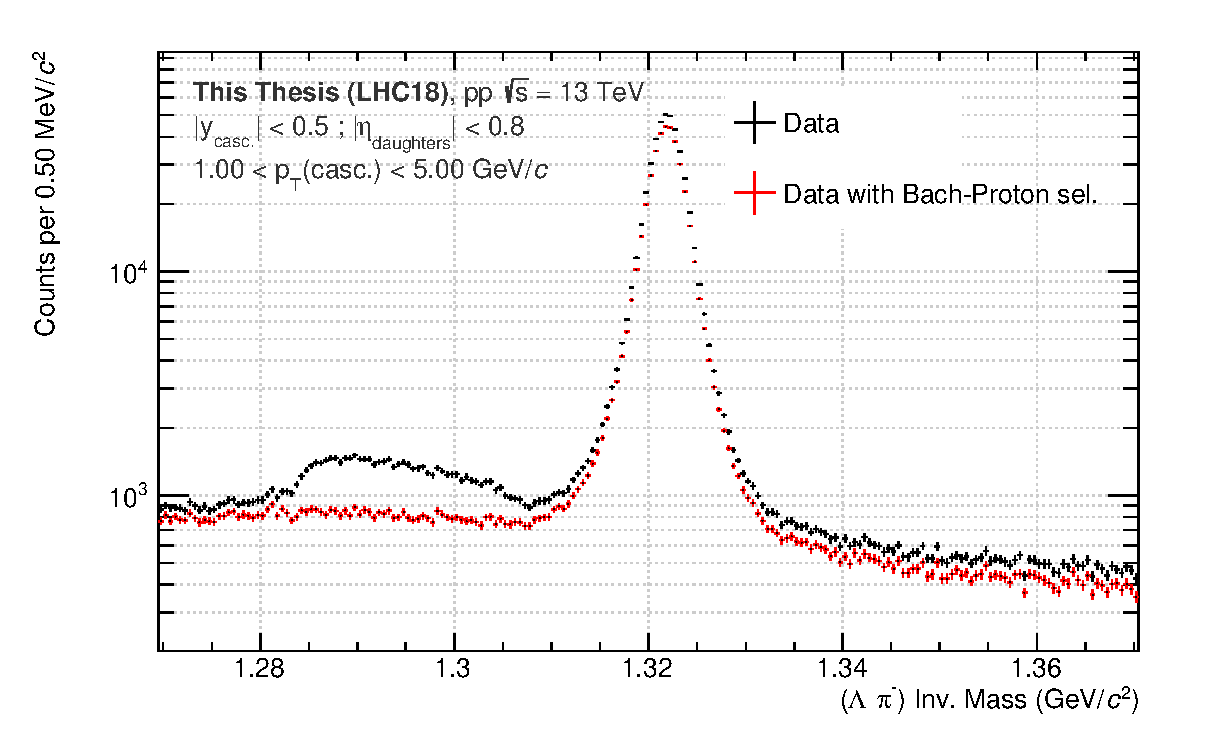
\includegraphics[width=0.6\textwidth]{Figs/Chapter5/InvMassXiMinus_WrongPA.eps}
	\label{fig:XiMinusWrongPA}
}
\subfigure[]
{
	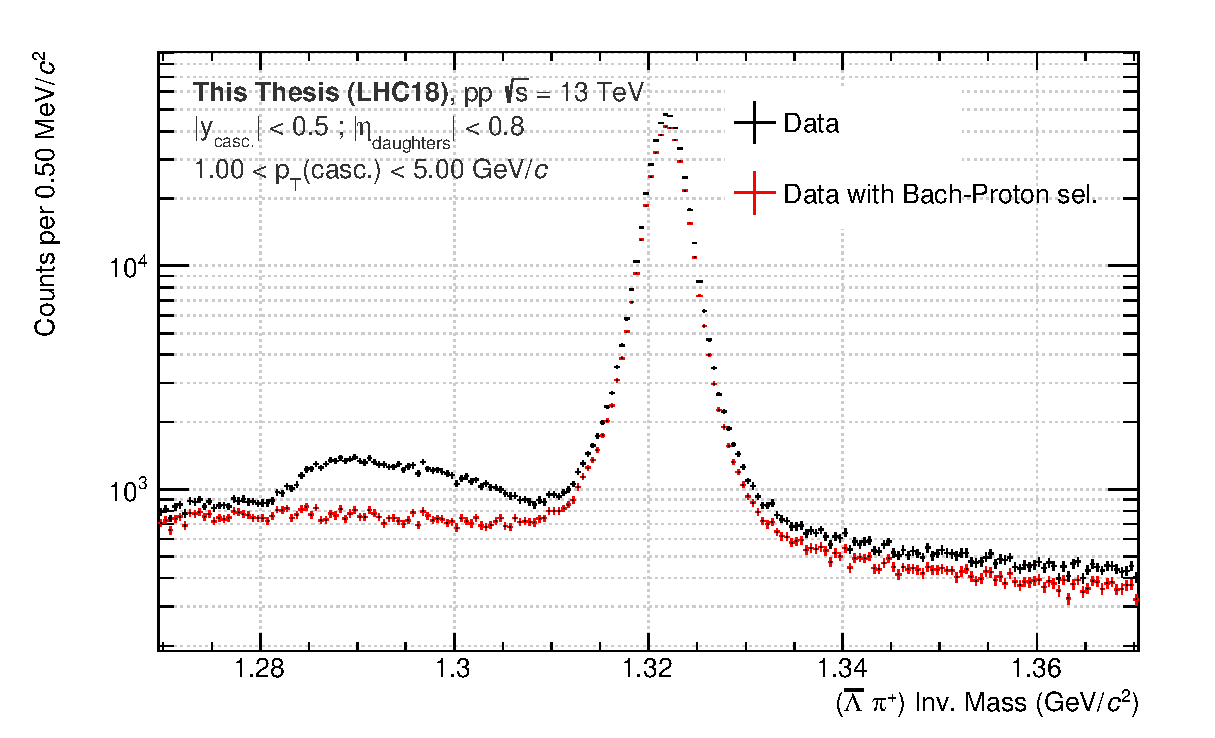
\includegraphics[width=0.6\textwidth]{Figs/Chapter5/InvMassXiPlus_WrongPA.eps}
	\label{fig:XiPlusWrongPA}
}
\hspace*{-1.5cm}	
\subfigure[]
{
	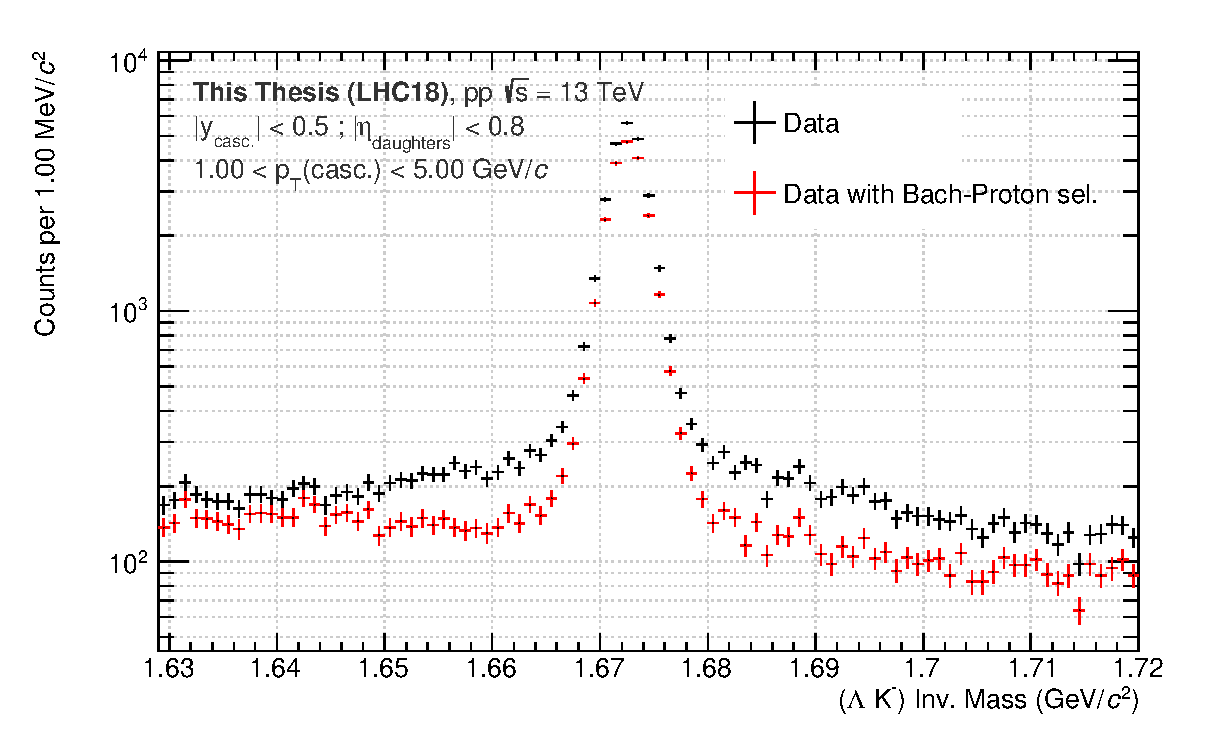
\includegraphics[width=0.6\textwidth]{Figs/Chapter5/InvMassOmegaMinus_WrongPA.eps}
	\label{fig:OmegaMinusWrongPA}
}
\subfigure[]
{
	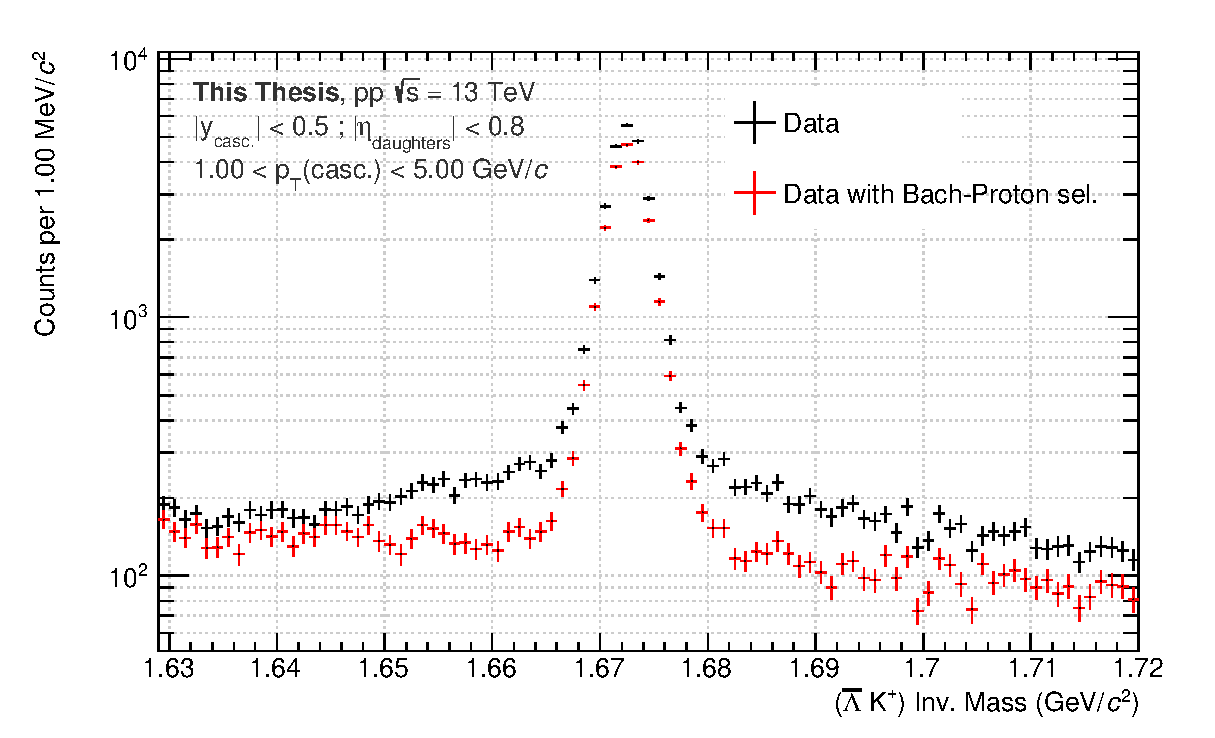
\includegraphics[width=0.6\textwidth]{Figs/Chapter5/InvMassOmegaPlus_WrongPA.eps}
	\label{fig:OmegaPlusWrongPA}
}	
	\caption{Invariant mass distribution of \rmXiM (a), \rmAxiP (b), \rmOmegaM (c) and \rmAomegaP (d) in pp at \sqrtS = 13 \tev. These have been obtained using the cuts in \tab\ref{tab:CascadeSelections} (red markers), except for the bachelor-proton pointing angle selection in black. This comparison shows the latter selection manages to remove a structure in the invariant mass distribution while preserving the population under the peak. Notice the log-scale on the y-axis, that puts into perspective the signal and background levels.}
	\label{fig:WrongPA}
\end{figure}

\begin{figure}[t]
%\centering
\hspace*{-2.cm}
\subfigure[]
{
	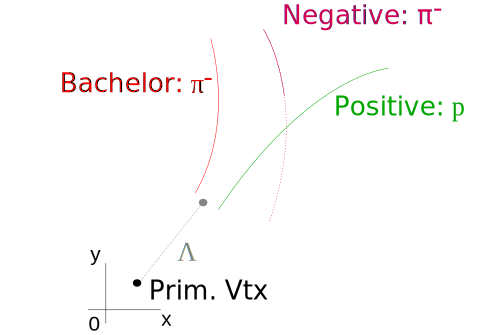
\includegraphics[width=0.32\textwidth]{Figs/Chapter5/WrongV0.png}
	\label{fig:WrongV0}
}
\subfigure[]
{
	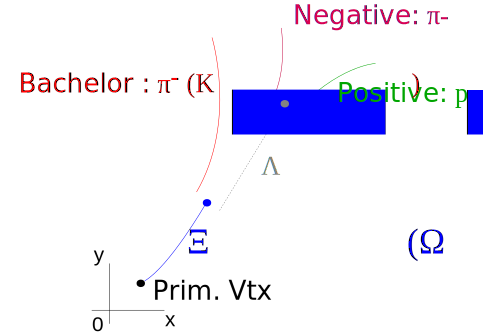
\includegraphics[width=0.32\textwidth]{Figs/Chapter5/TrueV0.png}
	\label{fig:TrueV0}
}
\subfigure[]
{
	\includegraphics[width=0.4\textwidth]{Figs/Chapter5/WrongPACut.png}
	\label{fig:WrongPACut}
}
	\caption{Invariant mass distribution of \rmXiM (a), \rmAxiP (b), \rmOmegaM (c) and \rmAomegaP (d) in pp at \sqrtS = 13 \tev. These have been obtained using the cuts in \tab\ref{tab:CascadeSelections} (red markers), except for the bachelor-proton pointing angle selection in black. This comparison shows the latter selection manages to remove a structure in the invariant mass distribution while preserving the population under the peak.}
	\label{fig:WrongTopology}
\end{figure}

\subsection{Mass measurement}
\label{subsec:MassExtraction}

\subsubsection{Principles of mass extraction}
\label{subsubsec:PrinciplesOfMassExtraction}

Out of all the candidates passing the above selection criteria, there contains true V0s/cascades -- depending on the particle of interest -- and background candidates. Taken individually, they are undistinguisable. The separation of these two can only be achieved statistically, based on the analysis of the invariant mass spectrum.

The invariant mass of each candidate is calculated, as explained in \Sec\ref{subsubsec:CascadeFormation} and \Sec\ref{subsubsec:InvariantMassSelection}, and sorted according to their electric charge in order to separate the particles from the anti-particles. The V0s being electrically neutral, they follow a different approach: since the \rmKzeroS decays into two particles of the same nature --- a \rmPiPlus and a \rmPiMinus ---, it is hopeless to try separating particles and anti-particles. This is not the case of \rmLambda and \rmAlambda, though. However, it may happen that the same V0 candidate passes the particle and anti-particle selections in \tab\ref{tab:V0Selections}. To avoid such double-counting, each candidate needs to go through the \rmLambda selections first. If it satisfies all conditions, it is labeled as \rmLambda and we move to the next candidate. Otherwise, it is checked against the requirements for a \rmAlambda baryon.

On one hand, most of the background candidates originate from a random association of two or three tracks. Those tracks being uncorrelated, the corresponding invariant mass spectrum should be flat or decreasing with the invariant mass value. On the other hand, the invariant mass of true V0s/cascades should be close to the tabulated mass \mPDG, such that there emerges an overpopulated region taking the shape of a peak. The \figs\ref{fig:InvMassCascades} show the invariant mass spectra of \rmXi and \rmOmega.  One can see that the signal for each species sits on top of a small background.\\

\begin{figure}[!t]
%\centering
\hspace*{-1.5cm}
\subfigure[]{
	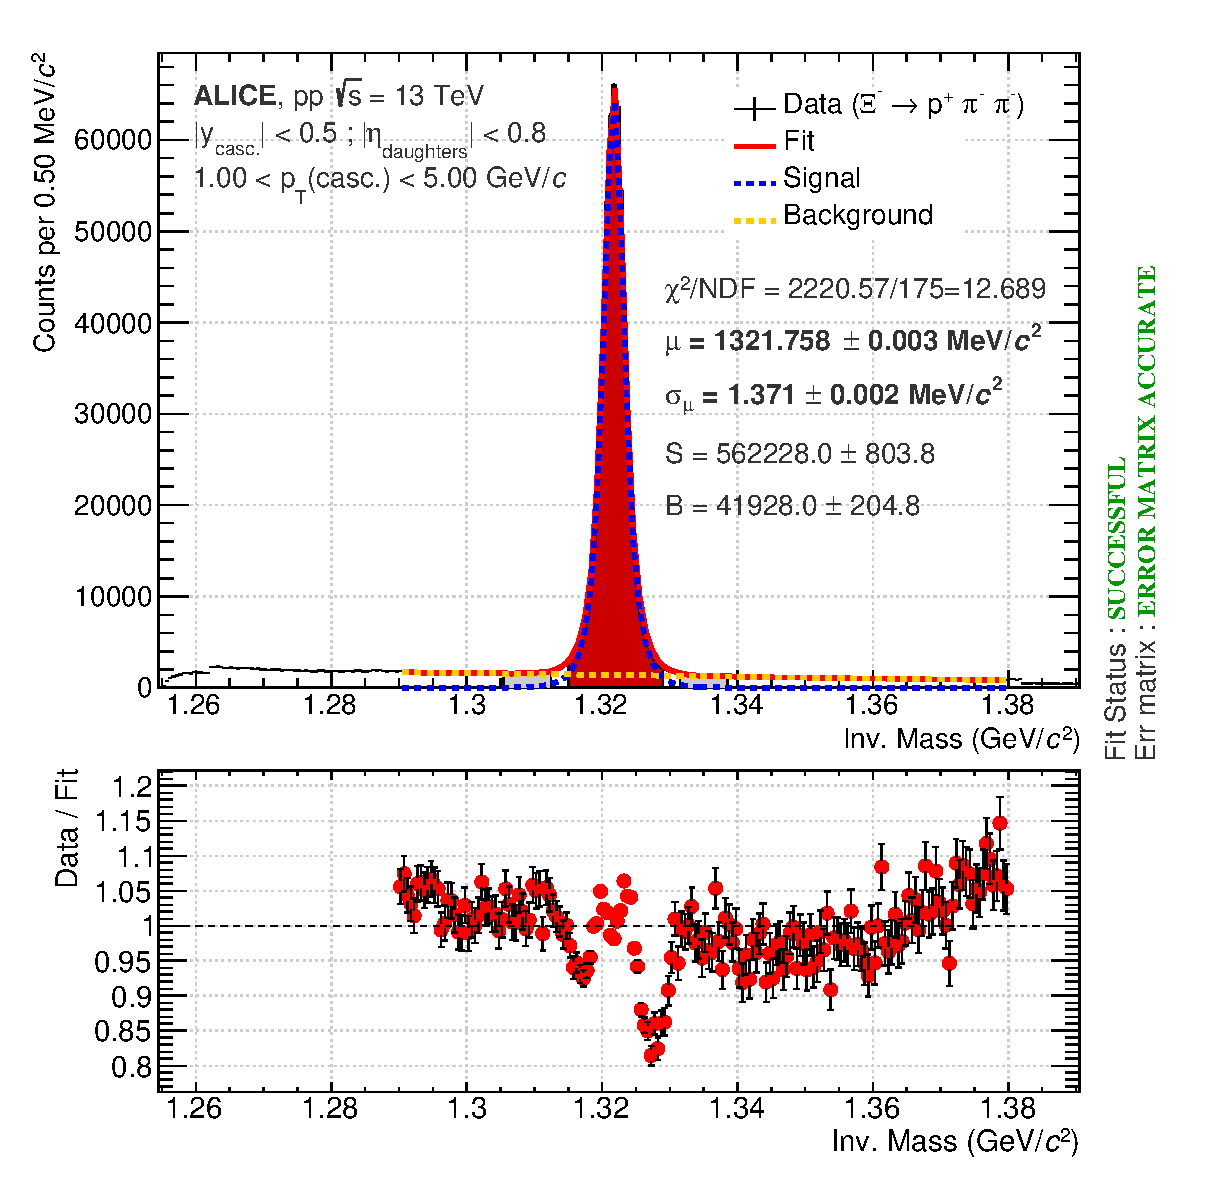
\includegraphics[width=0.6\textwidth]{Figs/Chapter5/InvMassXiMinus_ModifiedGaussian.eps}
	\label{fig:XiMinus_ModGaussian}
} 
\subfigure[]{
	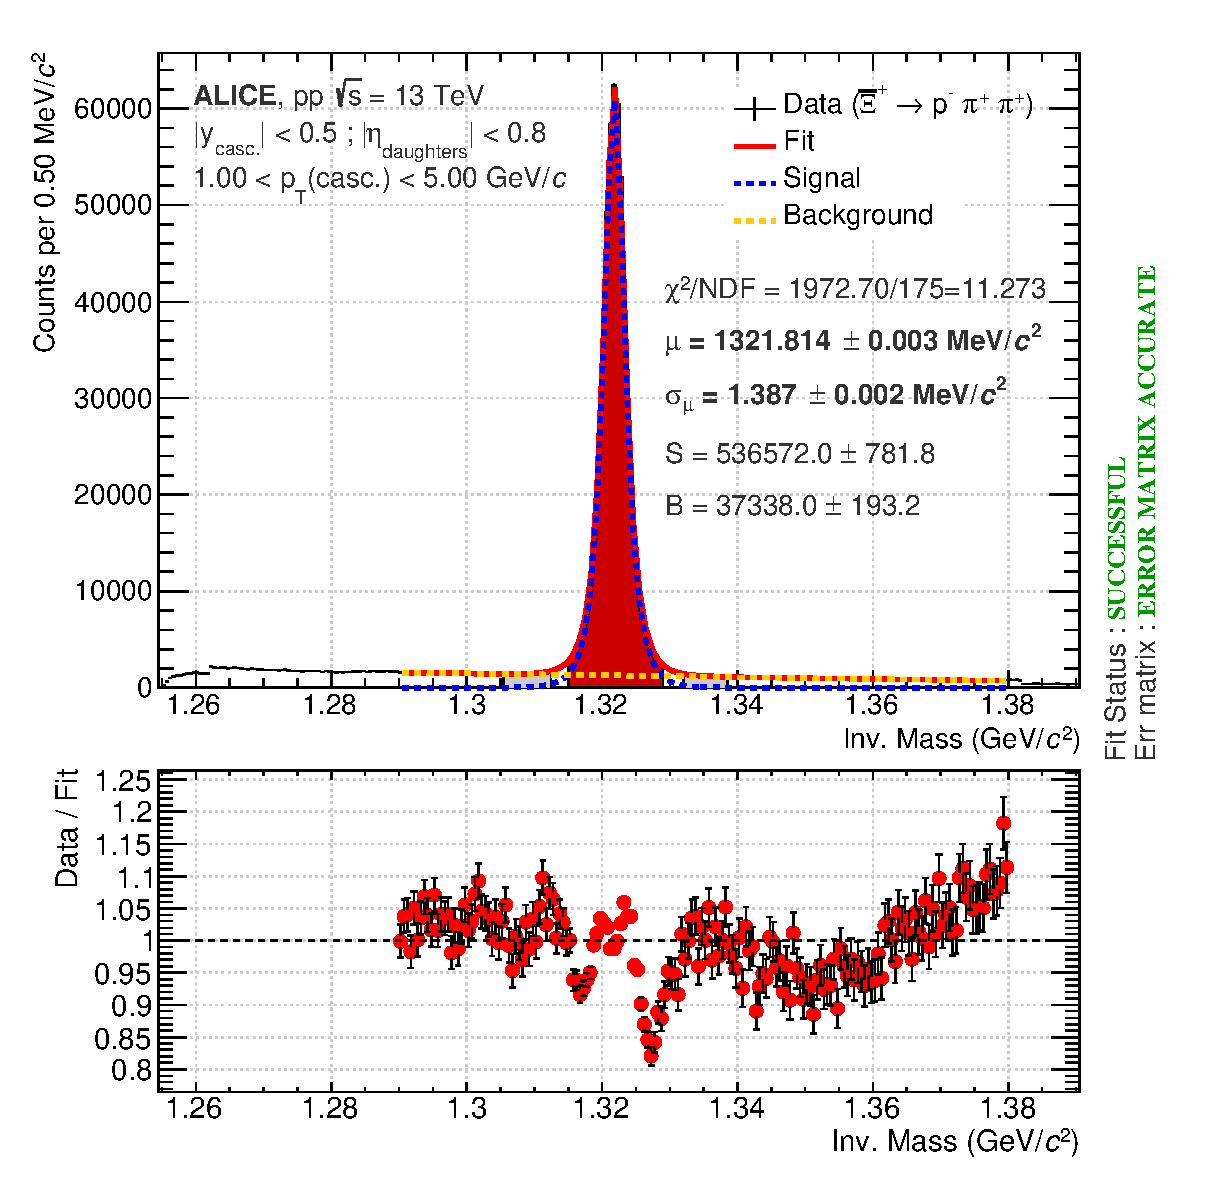
\includegraphics[width=0.6\textwidth]{Figs/Chapter5/InvMassXiPlus_ModifiedGaussian.eps}
	\label{fig:XiPlus_ModGaussian}
} 
\hspace*{-1.5cm}
\subfigure[]{
	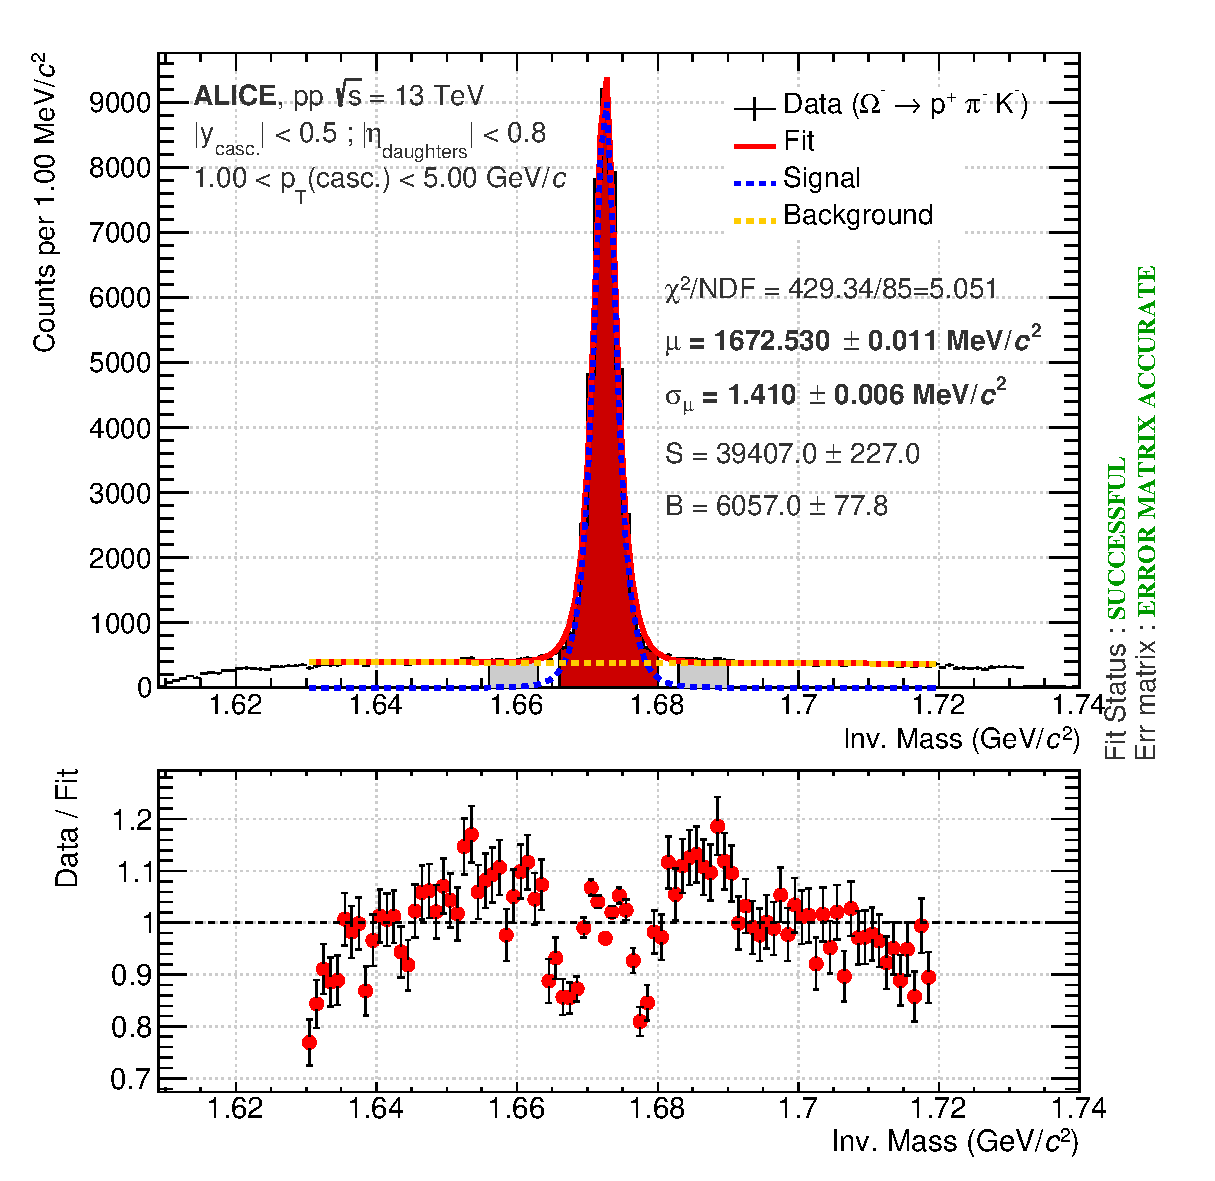
\includegraphics[width=0.6\textwidth]{Figs/Chapter5/InvMassOmegaMinus_ModifiedGaussian.eps}
	\label{fig:OmegaMinus_ModGaussian}
} 
\subfigure[]{
	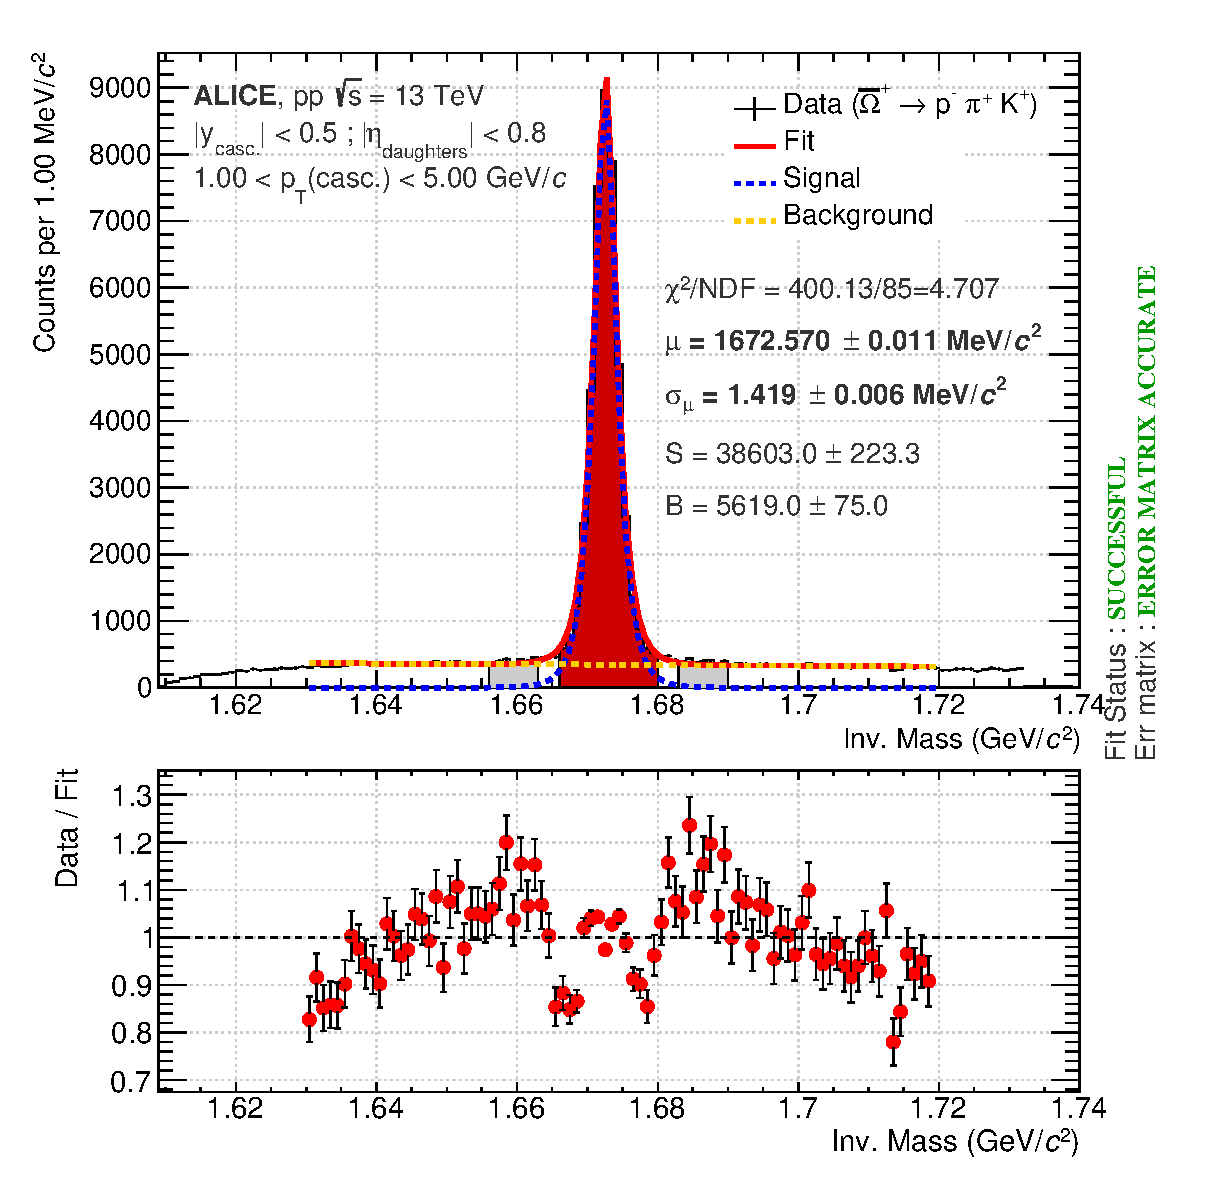
\includegraphics[width=0.6\textwidth]{Figs/Chapter5/InvMassOmegaPlus_ModifiedGaussian.eps}
	\label{fig:OmegaPlus_ModGaussian}
}  
\caption{Invariant mass distribution of \rmXiM (a), \rmAxiP (b), \rmOmegaM (c) and \rmAomegaP (d) hyperons in pp collisions at \sqrtS = 13 \tev. Here, the peak is modeled by a modified Gaussian, and the background by a first order polynomial. Each distribution comes with an additional panel representing consistency between the data and the fit model, in the form of a ratio. The error bars encompasses the uncertainties on both quantities.}
	\label{fig:InvMassCascades}
\end{figure}

To isolate the signal from the background, a fit of the invariant mass spectra is performed using the sum of two functions: one for modeling the signal peak, the other for describing the background. Several functions can be considered, as discussed in \Sec\ref{subsubsec:SignalBackShape}. In \figs\ref{fig:InvMassCascades}, the peak is represented by a modified Gaussian \cite{atlascollaborationKshortLambdaProduction2012} and the background by a linear function. Whatever their shape, the fitting procedure is performed with the maximum (log-)likelyhood method.

If the procedure manages to converge, this fit allows to measure the mass of the considered particle: it corresponds to the centre of the invariant mass peak, given by the position of the maximum of the signal function denoted as $\mu$. The width of the peak -- the parameter $\sigma$ -- provides an estimation of the mass resolution. The uncertainties on both quantities come from the errors returned by the fitting procedure.

From these parameters, two regions of interest can be delimited:
\begin{itemize}
\item[$\bullet$] the peak region, containing all the signal\footnote{More precisely, considering the definition of the peak region in this analysis, it should contain approximately 99.99995\% (\ie a $5 \sigma$ significance level) of the true V0s/cascades measured.} and some background, is defined in $\left[ \mu - 5 \sigma ; \mu + 5 \sigma \right]$;
\item[$\bullet$] the side-bands region, solely constituted of background, consists in two bands of the same width\footnote{As a side note: the two side-bands do not need to be of the same size, but it avoids dealing with a scaling factor when comparing their total area to the one in the peak region. Most often, they have different widths because of an asymmetry in the invariant mass distribution, such as the structure reported in \Sec\ref{subsubsec:InvMassStructure} \cite{alicecollaborationProductionLightflavorHadrons2020}.}, surrounding the peak region and covering the range $\left[ \mu - 12 \sigma ; \mu - 7 \sigma \right] \bigcup \left[ \mu + 7 \sigma ; \mu + 12 \sigma \right]$.
\end{itemize}
Hence, the amount of raw signal and background can be evaluated. The peak ($S+B$) and background ($B$) populations are estimated by counting the
number of candidates in their respective regions. The raw signal ($S$) in the peak region is obtained by subtracting the background from the peak population, that is $S = (S+B) - B$.

In \figs\ref{fig:InvMassCascades}, all the fit are of reasonably good quality. The mass peak sits on a small background; 1 237 666 $\pm$ 1162 \rmXiM (1 168 882 $\pm$ 1128 \rmAxiP) and 65 232 $\pm$ 277 \rmOmegaM (63 842 $\pm$ 274 \rmAomegaP) were reconstructed with purities above 90\%, as shown in \tab\ref{tab:FitQuantities}.

\begin{table}[h]
    \centering
    \begin{tabular}{b{5.35cm}@{\hspace{1cm}} b{2cm}@{\hspace{0.5cm}} b{2cm}@{\hspace{0.5cm}} b{1.5cm}@{\hspace{0.5cm}} b{1.5cm}@{\hspace{0.1cm}}}
    \noalign{\smallskip}\hline\noalign{\smallskip}
	Particle & \rmXiM & \rmAxiP & \rmOmegaM & \rmAomegaP \\	
    \noalign{\smallskip}\hline \noalign{\smallskip}
    Reduced $\chi^2$ & 12.689 & 11.273 & 5.051 & 4.707\\
    	Raw signal, $S$ &  1 237 666 & 1 168 882 & 65 232 & 63 842\\
    	Background, $B$ & 55 375 & 51 269 & 5758 & 5490 \\
    	$S/B$ & 22.4 & 22.8 & 11.4 & 11.7 \\
    	Purity, $S/(S+B)$ & 95.7\% & 95.8\% & 91.8\% & 92.1\% \\
    Signal significance, $S/\sqrt{S+B}$ & 1089 & 1059 & 245 & 243 \\
    \noalign{\smallskip}\hline\noalign{\smallskip}
    \end{tabular}
    \caption{Results from the fit of the invariant mass distributions in \fig\ref{fig:InvMassCascades} concerning the samples of \rmXiM, \rmAxiP, \rmOmegaM and \rmAomegaP. Therefore, this table reports the reduced $\chi^{2}$, raw signal, background, ratio $S/B$, purity and signal significance.}\label{tab:FitQuantities}
\end{table}

\subsubsection{Shape of the peak and background functions}
\label{subsubsec:SignalBackShape}

Since the mass extraction depends on the peak description, it is crucial to identify functional forms that reproduce accurately its shape. Different functions have been studied in MC simulations, based solely on true V0/cascade candidates. Thus, the invariant mass spectra contains no background candidates and follows approximately a Gaussian distribution centred on the injected mass, which usually corresponds to the PDG mass. The objective here is to define a list of functions, that fit correctly the invariant mass peak and thus display a good reduced $\chi^2$.


\begin{itemize}
\item[$\bullet$] \textbf{Symmetric function}: although the core of the invariant distribution exhibits an almost Gaussian shape due to the detector smearing, this is usually not the case for the tails. 

\begin{itemize}
\item \textbf{Triple Gaussian}: One option consists in taking the sum of an infinite number of Gaussians with a common mean. Here, three offer a reasonably good fit quality.
	\begin{equation}
	\dNdX{\mInv[]} = A_{1} \cdot \exp \left[ - \dfrac{ (\mInv[] - \mu )^2}{ 2 \sigma_{1}^2} \right] + A_{2} \cdot \exp \left[ - \dfrac{ (\mInv[] - \mu )^2}{ 2 \sigma_{2}^2} \right] + A_{3} \cdot \exp \left[ - \dfrac{ (\mInv[] - \mu )^2}{ 2 \sigma_{3}^2} \right]
	\label{eq:Gaus}
	\end{equation}
	with A the amplitude, $\mu$ the mean value of the distribution and $\sigma$ the width of the peak.
%	
%\item \textbf{Double Gaussian} : it consists in a sum of two Gaussian functions with different parameters but the mean value which is common.
%	\begin{equation}
%	\dNXdX{\rmXiPM(\rmOmegaPM)}{\mInvIdx{\rmLambdaPM \piPlusMinus (\rmLambdaPM \Kplusmin)}} = A_{1} \cdot \exp \left[ - \dfrac{ (\mInvIdx{\rmLambdaPM \piPlusMinus (\rmLambdaPM \Kplusmin)} - \mu )^2}{ 2 \sigma_{1}^2} \right] + A_{2} \cdot \exp \left[ - \dfrac{ (\mInvIdx{\rmLambdaPM \piPlusMinus (\rmLambdaPM \Kplusmin)} - \mu )^2}{ 2 \sigma_{2}^2} \right]
%	\end{equation}\label{eq:DoubleGaus}
%	where $A_1$ and $A_2$ are the respective amplitudes of the two Gaussian, $\mu$ corresponds to the center of the peak (common for the two Gaussian), and their widths are denoted as $\sigma_1$ and $\sigma_2$.
%	
\item \textbf{Modified Gaussian} \cite{atlascollaboration2012} : it provides a similar shape for the peak as the Double Gaussian, but with fewer parameters. Therefore, the fit procedure converges more easily and the \rmChiSquareNDF is generally smaller than with the Double Gaussian.
	\begin{equation}
	\dNdX{\mInv} = A \cdot \exp \left[ - \frac{1}{2} u^{1 + \frac{1}{1+ 0.5 u}} \right] \quad ; \quad  u = \left\rvert \frac{\mInv - \mu }{\sigma} \right\rvert
	\end{equation}\label{eq:ModifiedGaus}
	with $A$ the normalization, $\mu$ the mean, and $\sigma$ the width.
	
\end{itemize}

	\item[$\bullet$] \textbf{Asymmetric function}: Previous functions are all different flavours of Gaussian, and so are all symmetric. However, the tails of the invariant mass peak are not necessarly symmetric, and therefore asymmetric functions may be more suited for describing the peak.

	
	\begin{itemize}
\item \textbf{Bukin} \cite{bukin2007}\cite{niel2021} : the Bukin belongs to this class of functions. It has been built on the base of the convolution of a Gaussian and an exponential distributions.
	\begin{equation}
	\dNdX{\mInv} = 
		\begin{cases}
	      A \cdot \exp \left[ \rho_{\rm L} \frac{(u-x_{\rm L})^2}{(\mu-x_{\rm L})^2} - \ln(2) + 4 \cdot \ln(2)  \frac{(u-x_{\rm L})}{2 \sigma \sqrt{ 2  \ln 2 }} \cdot  \frac{\xi}{\sqrt{\xi^2+1} + \xi}  \frac{\sqrt{\xi^2+1}}{(\sqrt{\xi^2+1}-\xi)^2} \right], \qquad u\leq x_{\rm L} \\
	      \\
	      A \cdot \exp \left[ -\ln(2) \cdot \left( \frac{ \ln(1 + 4 \xi \sqrt{\xi^2+1} \frac{u - \mu}{2 \sigma \sqrt{2 \ln 2}}) }{ \ln( 1 + 2 \xi (\xi - \sqrt{\xi^2+1})) } \right)^2 \right], \qquad  x_{\rm L} < u < x_{\rm R} \\
	      \\
	      A \cdot \exp \left[ \rho_{\rm R} \frac{(u-x_{\rm R})^2}{(\mu-x_{\rm R})^2} - \ln(2) + 4 \cdot \ln(2) \frac{(u-x_{\rm R})}{2 \sigma \sqrt{ 2  \ln 2 }} \cdot  \frac{\xi}{\sqrt{\xi^2+1} + \xi} \frac{\sqrt{\xi^2+1}}{(\sqrt{\xi^2+1}-\xi)^2} \right], \qquad u \geq x_{\rm R} 
	     \end{cases}
	\end{equation}\label{eq:Bukin}
	with 
	\begin{equation}
		x_{\rm L, R} = \mu + \sigma \sqrt{ 2 \ln 2 } \left( \frac{ \xi}{ \sqrt{\xi^2 + 1 } } \mp 1 \right)
	\end{equation}
	where $u$ coincides with \mInv, $A$ is the normalization parameter, $\mu$ and $\sigma$ are the mean and the width of the peak, $\xi$ is an asymmetry parameter, $\rho_{\rm L}$ and $\rho_{R}$ are left and right exponential tail coefficients. The implementation has been taken from the \texttt{RooBukinPdf} class, in the \texttt{Roofit} package of ROOT \cite{verkerke2008}.

\end{itemize}

\end{itemize}



The origin of the data sample purity has to be found in the (very) tight cut on the cosine of pointing angle of the cascade candidate in \tab\ref{tab:CascadeSelections}. As a matter of fact, this selection has been tuned to reach such level of purity. Contrarily to the peak shape, the form of background is \textit{a priori} lesser known. For that reason, it is essential to control the level of background, and most particularly its profile, such that it can be modeled by one of the expected functional form.


For the background, two functional forms are studied :

\begin{itemize}
\item \textbf{Constant} : Combinatorial background is \textit{a priori} unstructured, so it can be approximated by a constant function.
\item \textbf{Linear} 
\end{itemize}

\subsubsection{Correction on the extracted mass}

Although the functions in \Sec\ref{subsubsec:SignalBackShape} describe well the invariant mass peak, the extracted mass does not agree with the injected mass, the PDG mass, as shown in \fig. This seemingly bias may stem from several elements. It can be due to the way data are processed, that might overestimate the reconstructed mass in a systematic manner. The analysis, and particularly the employed selections, may introduce a distortion in the invariant mass distribution, resulting in a different mass than the expected one. The fit procedure could also be the origin of such inconsistency; for instance, one of the tails may pre-dominate the procedure and drive the parameters in a certain direction.

Anyhow, in order to correct for any bias due to the data processing, the analysis or the fit procedure, an offset is applied on the extracted mass in simulated events such that it coincides with the injected value. It follows that this correction is then reported on the measured mass in real data. However, such a correction assumes a good agreement between the data and MC. To ensure that, the simulation is re-weighted to match the \pT spectra from the data.

This re-weighting procedure starts off by extracting the raw \pT spectra in the data. Similarly to the estimation of the amount of raw signal in \Sec\ref{subsubsec:PrinciplesOfMassExtraction}, the latter is given by subtracting the \pT spectrum in the side-bands region from the one in the peak region. It is then compared to the injected transverse momentum distribution of true V0/cascade candidates; the ratio of the \pT spectra in the data and MC provides the weighting factors.


\begin{figure}[!t]
%\centering
\hspace*{-1.5cm}
\subfigure[]{
	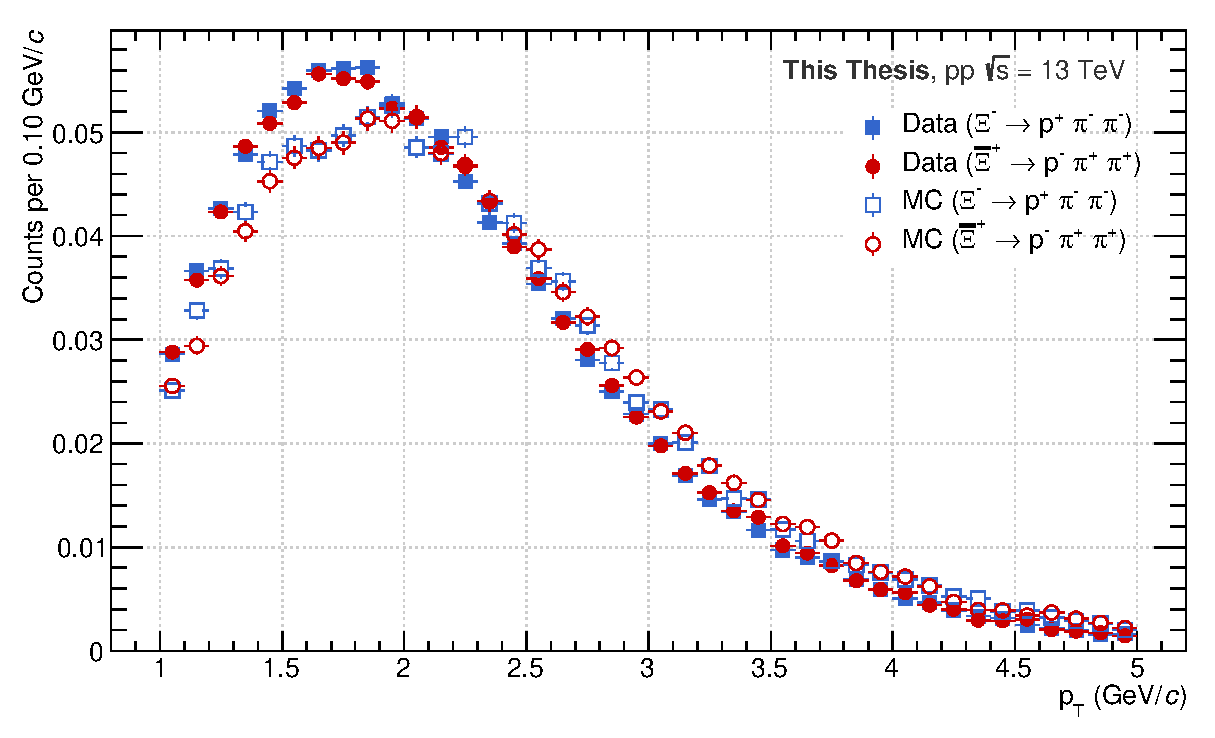
\includegraphics[width=0.6\textwidth]{Figs/Chapter5/RawPtSpectra_Xi.eps}
	\label{fig:XiMinus_ModGaussian}
} 
\subfigure[]{
	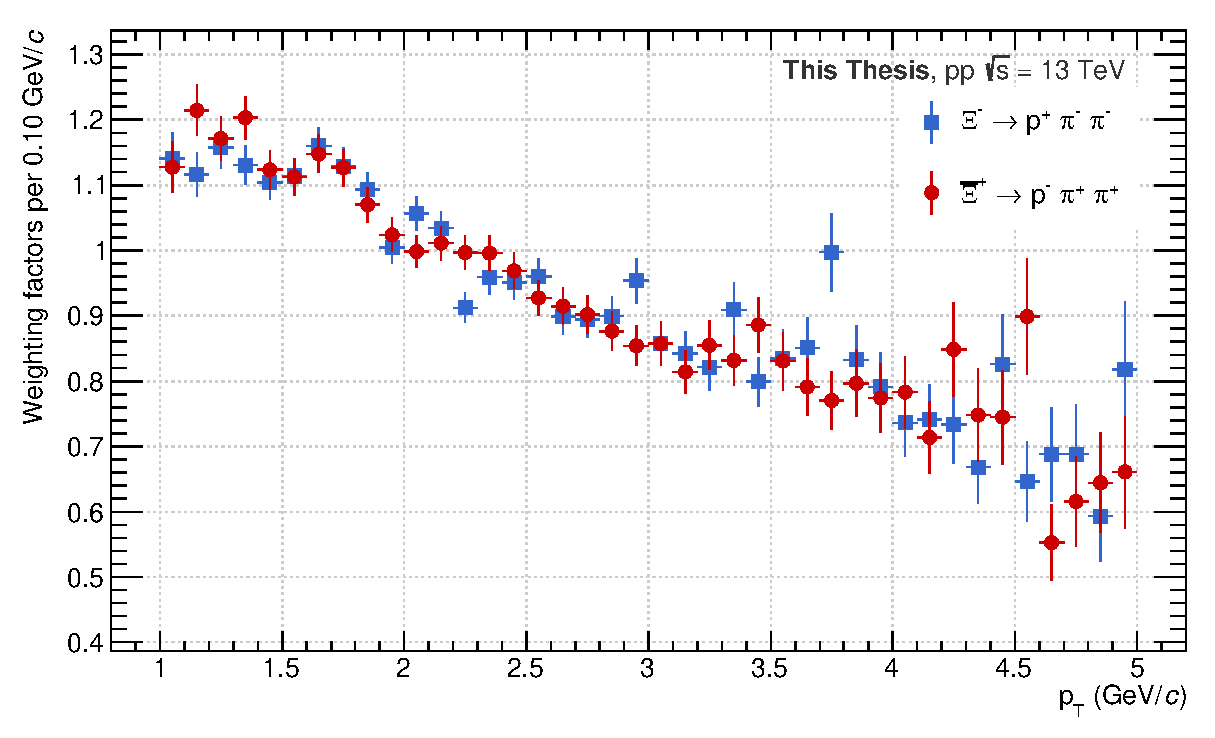
\includegraphics[width=0.6\textwidth]{Figs/Chapter5/WeightingFactors_Xi.eps}
	\label{fig:XiPlus_ModGaussian}
} 
\hspace*{-1.5cm}
\subfigure[]{
	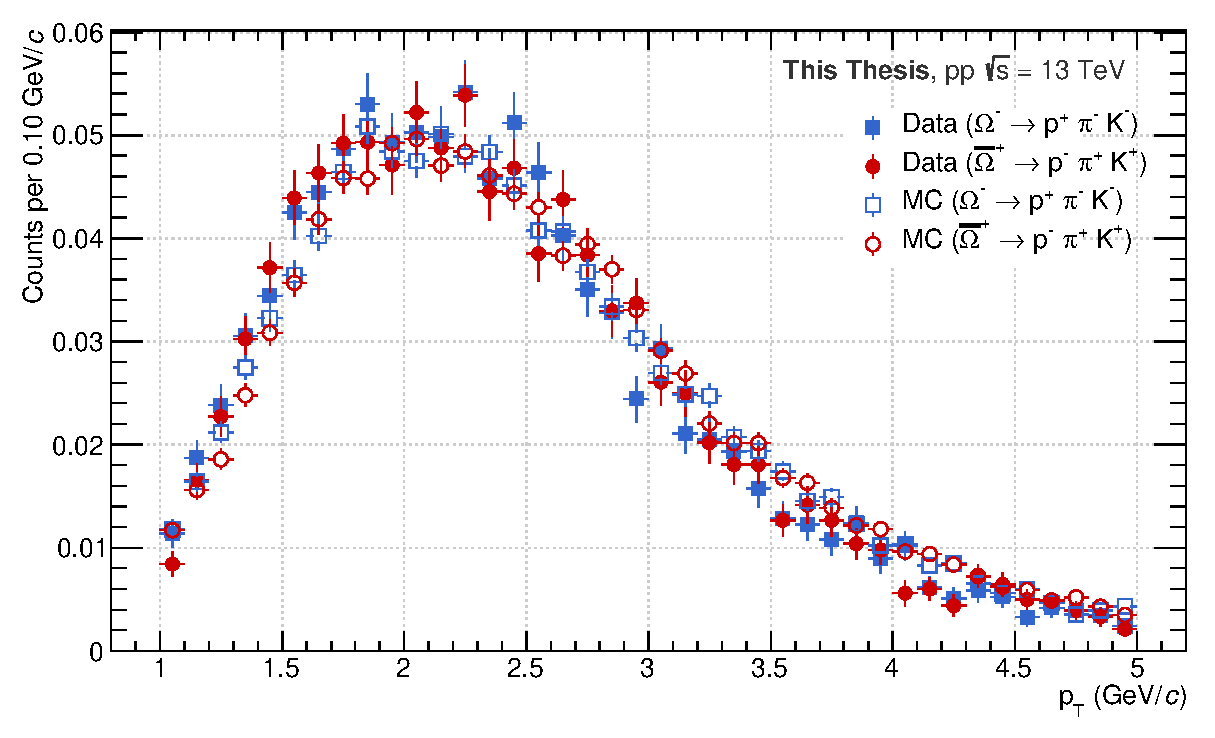
\includegraphics[width=0.6\textwidth]{Figs/Chapter5/RawPtSpectra_Omega.eps}
	\label{fig:OmegaMinus_ModGaussian}
} 
\subfigure[]{
	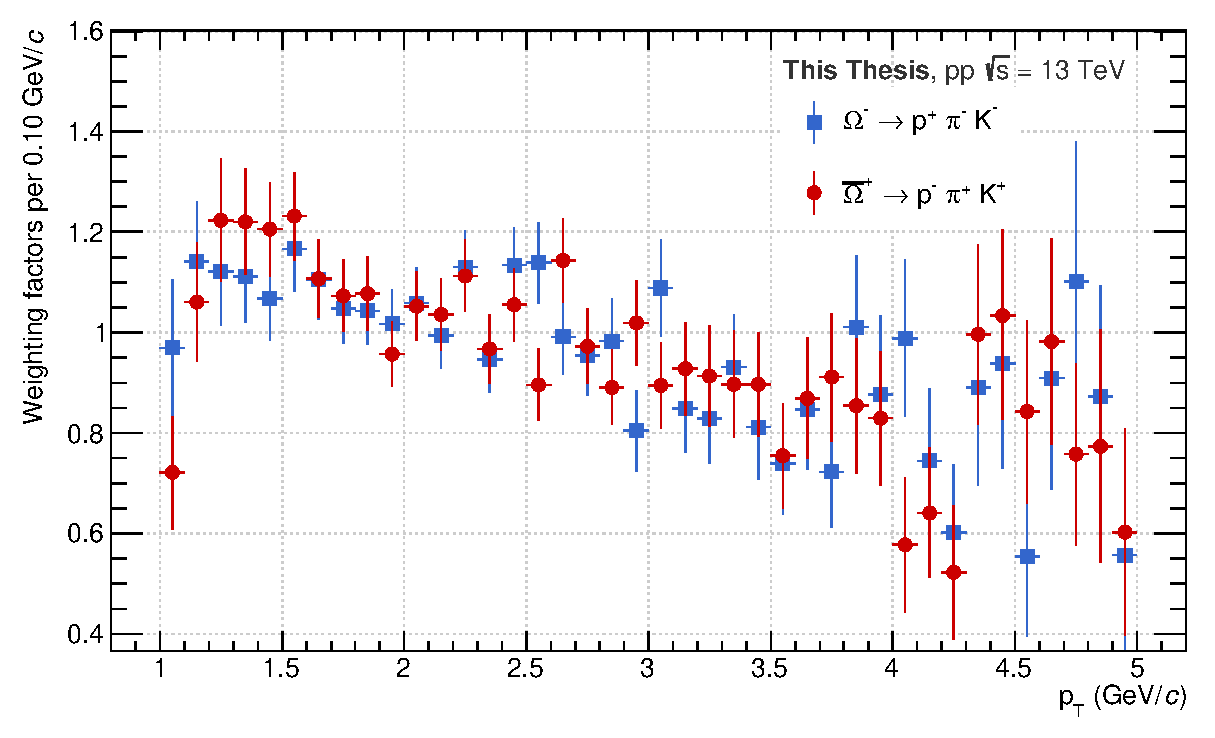
\includegraphics[width=0.6\textwidth]{Figs/Chapter5/WeightingFactors_Omega.eps}
	\label{fig:OmegaPlus_ModGaussian}
}  
\caption{Invariant mass distribution of \rmXiM (a), \rmAxiP (b), \rmOmegaM (c) and \rmAomegaP (d) hyperons in pp collisions at \sqrtS = 13 \tev. Here, the peak is modeled by a modified Gaussian, and the background by a first order polynomial. Each distribution comes with an additional panel representing consistency between the data and the fit model, in the form of a ratio. The error bars encompasses the uncertainties on both quantities.}
	\label{fig:PtSpectra}
\end{figure}


Once the simulated data have been re-weighted, the mass offset observed in MC with respect to the injected mass is assessed, corrected and taken into account in the mass measurement in real data. The \tab\ref{tab:MCMassOffset} presents these corrections as well as the corrected mass values. From these derive the (relative) mass difference between particle and anti-particle, given by
\begin{equation}
\frac{\Delta \mu}{\mu}=  \frac{\mu_{\overline{\textsc{part.}}} - \mu_{\textsc{part.}}}{\mu_{\textsc{part.}}}.
\end{equation}
The \tab\ref{tab:MCMassDiffOffset} shows mass difference for \rmXi and \rmOmega, in the data and MC, as well as the corrected value.

\begin{table}[!h]
    \centering
    \footnotesize
    \begin{tabular}{b{2.5cm}@{\hspace{0.5cm}} b{2.5cm}@{\hspace{0.5cm}} b{2.5cm}@{\hspace{0.5cm}} b{2.5cm}@{\hspace{0.5cm}} b{2.5cm}@{\hspace{0.5cm}}}
    \noalign{\smallskip}\hline\noalign{\smallskip}
    \bf Particle & \bf \rmXiM & \bf \rmAxiP & \bf \rmOmegaM & \bf \rmAomegaP \\
    \noalign{\smallskip}\hline \noalign{\smallskip}    
    Offset in data & $0.004 \pm 0.004$  & $0.055\pm 0.004$ & $0.090\pm 0.014$ & $0.066 \pm 0.014$ \\
    Offset in MC & $-0.127 \pm 0.003$  & $-0.125\pm 0.003$ & $-0.023\pm 0.004$ & $-0.005 \pm 0.004$ \\
    	Corrected mass & $1321.841 \pm 0.005$ & $1321.890 \pm 0.005$ & $1672.517 \pm 0.015$ & $1672.511 \pm 0.015$\\
    \noalign{\smallskip}\hline\noalign{\smallskip}
    \end{tabular}
    \caption{Measurements of the mass offset with respect to the PDG value (coinciding with the injected mass in MC) in the data and MC, as well as the final corrected masses of $\Xi^{-}$, $\overline{\Xi}^{+}$, $\Omega^{-}$, $\overline{\Omega}^{+}$. The uncertainties on the mass values correspond only to the statistical one. These measurements have been obtained using the selections in \tab\ref{tab:CascadeSelections}, a modified Gaussian for the peak modelisation and a linear function for the background (in the data only).}\label{tab:MCMassOffset}
\end{table}

\begin{table}[!h]
    \centering
%    \footnotesize
    \begin{tabular}{b{7.5cm}@{\hspace{0.5cm}} b{3cm}@{\hspace{0.5cm}} b{3cm}@{\hspace{0.5cm}}}
    	\noalign{\smallskip}\hline \noalign{\smallskip}    
    \bf Particle & \bf \rmXi & \bf \rmOmega\\
    \noalign{\smallskip}\hline \noalign{\smallskip}  
    Mass difference offset in data ($\times 10^{-5}$) & $0.004 \pm 0.004$  & $0.004 \pm 0.004$ \\
    Mass difference offset in MC ($\times 10^{-5}$)& $0.004 \pm 0.004$ & $0.004 \pm 0.004$  \\
    	Corrected mass difference ($\times 10^{-5}$) & $0.004 \pm 0.004$ & $0.004 \pm 0.004$ \\
    
    \noalign{\smallskip}\hline\noalign{\smallskip}
    \end{tabular}
    \caption{Measurements of the mass difference in the data and MC, as well as the final corrected mass difference for $\Xi^{\pm}$ and $\Omega^{\pm}$. The uncertainties on the mass differences correspond only to the statistical one. These measurements have been obtained using the selections in \tab\ref{tab:CascadeSelections}, a modified Gaussian for the peak modelisation and a linear function for the background (in the data only).} 
    \label{tab:MCMassDiffOffset}
\end{table}

\section{Study of the systematic uncertainties}

A systematic study consists in reviewing an analysis via the test of its different elements. It involves identifying the source of systematic errors that might affect the values of the extracted mass and their corresponding uncertainties. Usually, this is achieved by repeating the analysis with a few minor changes, in the hope that there will be no effect. If that is the case, meaning that the obtained values are consistent, then one could argue that the analysis is free of systematic effect and under control: no additional measure are requested. On the contrary, a large deviation in the values indicates the presence of a systematic effect, that should be treated seriously. 

In pratice, one needs to define what "small" and "large" deviations mean. If an analysis is performed in two different ways: the first approach gives the result $a_1$ with an uncertainty $\sigma_1$ ; the second $a_2$ with an uncertainty $\sigma_2$. The difference between the results is given by $\Delta = a_1 - a_2$ and the error on the difference by $\sigma_{\Delta} = \sqrt{ |\sigma_{1}^{2} - \sigma_{2}^{2} | }$. If the ratio $\Delta/\sigma_{\Delta}$ is greater than a certain threshold value -- denoted \sigmaBarlow and to be defined by the analyser --, this points out a systematic effect that requires further investigation. This approach is known as the \textit{Barlow criterion}.

As in cooking, what separates the good systematic study from the lesser good one is the choice of the seasoning, namely the choice of the threshold value. The larger the \sigmaBarlow, the more systematic effects would slip under the radar; conversely, the smaller the threshold, the higher the sensitivity to the systematic effects. Since the targeted precision on the mass and mass difference values is very low, the systematic effects must be well under control. Therefore, in the context of this analysis, the contribution of a potential source of systematics is said to be significant for $\sigmaBarlow\simeq 1$. \\

However, the presence of a systematic effect does not necessarily imply a systematic uncertainty. In fact, there are two possibilites. Either a systematic correction can be applied and the error on that correction will be quoted as the systematic uncertainty, or the correction may be difficult (or impossible) to derive and therefore the systematic uncertainty will have to fully encompass the imprecision induced to the systematic effect.

This treatement of the systematics corresponds to the one proposed by Roger Barlow \cite{barlow2000}\cite{barlow2002}. The following section presents the list of systematic sources studied for this analysis, with their estimated uncertainties or corrections.

\subsection{Topological and track selections}

As explained in \Sec\ref{subsec:TopoReco}, the identification of the charged \rmXi and \rmOmega baryons relies on their characteristic cascade decay. The reconstruction of these decay topology revolves around, first, the association of two tracks to form \rmLambda candidates, and then these are matched with the remaining secondary tracks. In order to reduce the induced combinatorial background, various topological and kinematic cuts are being used. The choice of the employed cut values may obviously be the source of a bias. Such a systematic effect can be revealed by observing a variation of the mass and/or its uncertainty under a different set of selections.

The standard approach consists in varying individually each selection, while keeping the others at their reference value. Although it allows to address the bias induced by a given cut, this does not take into account the correlations between topological variables. For instance, a higher cut on cascade decay radius also implies that the \rmLambda daughter decays further away in the detector. To tackle that, one needs to build a matrix containing the correlation factors for each pair of selection variables.

However, a different approach is followed here. To go over the correlations between each variable, the sets of selections are randomly generated according to an uniform law, that spans over a certain variation range. 


\begin{table}[h]
    \centering
    \begin{tabular}{c|c|c}
    \noalign{\smallskip}\hline \noalign{\smallskip}
    \bf Track variable & Range & Signal variation \rmXiM (\rmAxiP) \\
    \noalign{\smallskip}\hline \noalign{\smallskip}
    Nbr of crossed TPC readout rows & $> \left[ 70 ; 90 \right]$ &  1\% (1\%)\\
    $\Nsigma^{\rm TPC}$ & $<\left[ 1 ; 3 \right] $ &  60\% (60\%)\\
    
    \noalign{\smallskip}\hline \noalign{\smallskip}
    \bf Topological variable & Range & Signal variation \rmXiM (\rmAxiP) \\
    \noalign{\smallskip}\hline \noalign{\smallskip}
    
    \multicolumn{3}{l}{\textbf{V0}} \\
    V0 decay radius (\cm) & $> \left[ 1.2 ; 8 \right]$ & 11\% (11\%)\\
    V0 cosine of pointing angle & $> \left[ 0.97 ; 0.998 \right]$ & 10\% (10\%)\\
    |$m$($V0$) - \mPDG\rmLambda| (\gmass) & $< \left[ 0.002 ; 0.007 \right]$ & 18\% (18\%)\\
    DCA proton to prim. vtx (\cm) & > $\left[ 0.04 ; 0.5 \right]$ & 28\% (28\%)\\
    DCA pion to prim. vtx (\cm) & > $\left[ 0.04 ; 0.95 \right]$ & 10\% (10\%)\\
    DCA V0 to prim. vtx (\cm) & > $\left[ 0.06 ; 0.2 \right]$ & 12\% (12\%)\\
    DCA between V0 daughters (std dev) & < $\left[ 0.4 ; 1.2 \right]$ & 12\% (12\%) \\
    \noalign{\smallskip}\hline \noalign{\smallskip}
    
    \multicolumn{3}{l}{\textbf{Cascade}} \\
    Cascade decay radius (\cm) & > $\left[ 0.5 ; 2.5 \right]$ & 11\% (11\%)\\
    Cascade Lifetime (\cm) & < $\left[ 1.6 ; 3.40 \right]$ \cTau & 40\% (40\%)\\
    DCA bachelor to prim. vtx (\cm) & > $\left[ 0.04 ; 0.5 \right]$ & 15\% (15\%) \\
    DCA between the cascade daughters (std dev) & < $\left[ 0.25 ; 1.2 \right]$ & 12\% (12\%)\\
    Cascade cosine of pointing angle & > $\left[ 0.995 ; 0.9995 \right]$ & 14\% (14\%)\\
    Bachelor-proton pointing angle (rad) & > $\left[ 0.02 ; 0.05 \right]$ & 11\% (11\%) \\
    
    \noalign{\smallskip}\hline \noalign{\smallskip}
    \end{tabular}
    \caption{Summary of the range variation on the topological and track selections used for the reconstruction of \rmXiM and \rmAxiP. The induced signal variation is indicated in the last column ; for more details, look at \fig\ref{fig:SignalVariation_TopoSel_XiMinus} and \fig\ref{fig:SignalVariation_TopoSel_XiPlus}.}\label{tab:SystematicSelectionsXi}
\end{table}

\begin{table}[h]
    \centering
    \begin{tabular}{c|c|c}
    \noalign{\smallskip}\hline \noalign{\smallskip}
    \bf Candidate variable & Range & Signal variation \rmOmegaM (\rmAomegaP) \\
    \noalign{\smallskip}\hline \noalign{\smallskip}    
    Competing mass rejection (\gmass) & $> \left[ 0.006 ; 0.010 \right]$ & 0.9\% (0.9\%)\\
    
    \noalign{\smallskip}\hline \noalign{\smallskip}
    \bf Track variable & Range & Signal variation \rmOmegaM (\rmAomegaP) \\
    \noalign{\smallskip}\hline \noalign{\smallskip}
    Nbr of crossed TPC readout rows & $> \left[ 70 ; 90 \right]$ &  2.5\% (2.5\%)\\
    $\Nsigma^{\rm TPC}$ & $< \left[ 1 ; 3 \right] $ &  60\% (60\%)\\
    
    \noalign{\smallskip}\hline \noalign{\smallskip}
    \bf Topological variable & Range & Signal variation \rmOmegaM (\rmAomegaP) \\
    \noalign{\smallskip}\hline \noalign{\smallskip}
    
    \multicolumn{3}{l}{\textbf{V0}} \\
    V0 decay radius (\cm) & $> \left[ 1 ; 5.5 \right]$ & 11\% (11\%)\\
    V0 cosine of pointing angle & $> \left[ 0.97 ; 0.998 \right]$ & 17\% (17\%)\\
    |$m$($V0$) - \mPDG\rmLambda| (\gmass) & $< \left[ 0.002 ; 0.007 \right]$ & 17\% (17\%)\\
    DCA proton to prim. vtx (\cm) & $> \left[ 0.04 ; 0.5 \right]$ & 34\% (34\%)\\
    DCA pion to prim. vtx (\cm) & $> \left[ 0.04 ; 0.75 \right]$ & 10\% (10\%) \\
    DCA V0 to prim. vtx (\cm) & $> \left[ 0.06 ; 0.2 \right]$ & 14\% (14\%)\\
    DCA between V0 daughters (std dev) & $< \left[ 0.4 ; 1.2 \right]$ & 11\% (11\%)\\
    \noalign{\smallskip}\hline \noalign{\smallskip}
    
    \multicolumn{3}{l}{\textbf{Cascade}} \\
    Cascade decay radius (\cm) & $> \left[ 0.5 ; 1.6 \right]$ & 12\% (12\%)\\
    Cascade Lifetime (\cm) & $< \left[ 1.6 ; 3.40 \right]$ \cTau & 14\% (14\%)\\
    DCA bachelor to prim. vtx (\cm) & $> \left[ 0.05 ; 0.2 \right]$ & 13\% (13\%)\\
    DCA between the cascade daughters (std dev) & $< \left[ 0.15 ; 1.2 \right]$ & 12\% (12\%)\\
    Cascade cosine of pointing angle & $> \left[ 0.995 ; 0.9995 \right]$ & 17\% (17\%)\\
    Bachelor-proton pointing angle & $> \left[ 0.02 ; 0.05 \right]$ & 13\% (13\%)\\
    
    \noalign{\smallskip}\hline \noalign{\smallskip}
    \end{tabular}
    \caption{Summary of the range variation on the topological and track selections used for the reconstruction of \rmOmegaM and \rmAomegaP. The induced signal variation is indicated in the last column ; for more details, look at \fig\ref{fig:SignalVariation_TopoSel_OmegaMinus} and \fig\ref{fig:SignalVariation_TopoSel_OmegaPlus}.}\label{tab:SystematicSelectionsOmega}
\end{table}

\begin{table}[h]
    \centering
    \begin{tabular}{c|c|c}
    \noalign{\smallskip}\hline \noalign{\smallskip}
    \bf Candidate variable & Range & Signal variation \rmKzeroS \\
    \noalign{\smallskip}\hline \noalign{\smallskip}    
    Competing mass rejection (\gmass) & $> \left[ 0.002 ; 0.010 \right]$ & 1.1\% \\
    
    \noalign{\smallskip}\hline \noalign{\smallskip}
    \bf Track variable & Range & Signal variation \rmKzeroS \\
    \noalign{\smallskip}\hline \noalign{\smallskip}
    Nbr of crossed TPC readout rows & $> \left[ 70 ; 90 \right]$ &  0.5\% \\
    $\Nsigma^{\rm TPC}$ & $< \left[ 1 ; 3 \right] \ \sigma$ &  45\% \\
    
    \noalign{\smallskip}\hline \noalign{\smallskip}
    \bf Topological variable & Range & Signal variation \rmKzeroS \\
    \noalign{\smallskip}\hline \noalign{\smallskip}
    
    V0 decay radius (\cm) & $> \left[ 0.4 ; 2.2 \right]$ & 10\% \\
    V0 Lifetime (\cm) & $< \left[ 1.57 ; 3.43 \right]$ \cTau & 12\% \\
    V0 cosine of pointing angle & $> \left[ 0.995 ; 0.9998 \right]$ & 10\% \\
    DCA pion to prim. vtx (\cm) & $> \left[ 0.04 ; 0.5 \right]$ & 24\% \\
%    DCA V0 to prim. vtx (\cm) & < $\left[ 0.04 ; 1 \right]$ & 35\% \\
    DCA between V0 daughters (std dev) & $< \left[ 0.2 ; 1.5 \right]$ & 12\%\\
    \noalign{\smallskip}\hline \noalign{\smallskip}
    \end{tabular}
    \caption{Summary of the range variation on the topological and track selections used for the reconstruction of \rmKzero. The induced signal variation is indicated in the last column ; for more details, look at \fig\ref{fig:SignalVariation_TopoSel_K0s}.}\label{tab:SystematicSelectionsK0s}
\end{table}

\begin{table}[h]
    \centering
    \begin{tabular}{c|c|c}
    \noalign{\smallskip}\hline \noalign{\smallskip}
    \bf Candidate variable & Range & Signal variation \rmLambda (\rmAlambda) \\
    \noalign{\smallskip}\hline \noalign{\smallskip}    
    Competing mass rejection (\gmass) & > $\left[ 0.005 ; 0.012 \right]$ & 3\% (3\%)\\
    
    \noalign{\smallskip}\hline \noalign{\smallskip}
    \bf Track variable & Range & Signal variation \rmLambda (\rmAlambda) \\
    \noalign{\smallskip}\hline \noalign{\smallskip}
    Nbr of crossed TPC readout rows & > $\left[ 70 ; 90 \right]$ &  0.8\% (0.8\%)\\
    $\Nsigma^{\rm TPC}$ & < $\left[ 1 ; 3 \right] \ \sigma$ &  45\% (45\%)\\
    
    \noalign{\smallskip}\hline \noalign{\smallskip}
    \bf Topological variable & Range & Signal variation \rmLambda (\rmAlambda) \\
    \noalign{\smallskip}\hline \noalign{\smallskip}
    
    V0 decay radius (\cm) & $> \left[ 0.4 ; 3.5 \right]$ & 11\% (11\%)\\
    V0 Lifetime (\cm) & $< \left[ 1.53 ; 3.43 \right]$ \cTau & 17\% (17\%)\\
    V0 cosine of pointing angle & $> \left[ 0.995 ; 0.9998 \right]$ & 13\% (13\%)\\
    DCA proton to prim. vtx (\cm) & $> \left[ 0.04 ; 0.15 \right]$ & 17\% (17\%)\\
    DCA pion to prim. vtx (\cm) & $> \left[ 0.04 ; 0.5 \right]$ & 12\% (12\%) \\
%    DCA V0 to prim. vtx (\cm) & $< \left[ 0.06 ; 0.2 \right]$ & 25\% (25\%)\\
    DCA between V0 daughters (std dev) & $< \left[ 0.3 ; 1.5 \right]$ & 12\% (12\%)\\ 
    \noalign{\smallskip}\hline \noalign{\smallskip}
    \end{tabular}
    \caption{Summary of the range variation on the topological and track selections used for the reconstruction of \rmLambda and \rmAlambda. The induced signal variation is indicated in the last column ; for more details, look at \fig\ref{fig:SignalVariation_TopoSel_Lambda} and \fig\ref{fig:SignalVariation_TopoSel_AntiLambda}.}\label{tab:SystematicSelectionsLambda}
\end{table}

\subsubsection{Influence on the mass extraction}

\subsubsection{Influence on the mass difference mass}

\subsection{Momentum scale}

\subsubsection{Energy loss corrections}

\subsubsection{Imprecision on the magnetic field}

\subsection{Pile-up treatment}

\subsection{Mass extraction}

\subsubsection{Choice of the fit function}

\subsubsection{Choice of the fitting range}

\subsubsection{Choice of the binning}

\subsection{Correction on the extracted mass}

\subsection{Precision on the tabulated masses}

\subsection{Other possible biases}

\section{Results}